\documentclass[a4paper, 11pt]{article}
\usepackage[ngerman]{babel}
%ä und so
\usepackage[utf8]{inputenc}
\usepackage[T1]{fontenc}
\usepackage{amsmath}
\usepackage{amsthm}
\usepackage{amsbsy}

\usepackage{mathrsfs}
\usepackage{amssymb}
\usepackage{amstext}
\usepackage{amsfonts}
\usepackage{float}
\usepackage{graphicx}
\usepackage{esdiff}
\usepackage{hyperref}
\usepackage{geometry}
\geometry{top = 20mm, bottom = 20 mm, left = 25mm, right = 25mm}


\usepackage{setspace}
\onehalfspacing

\usepackage{fancyhdr}
\usepackage{wrapfig}
%\usepackage[hyphens]{url}
%\urlstyle{sf}
%\usepackage[hidelinks]{hyperref}
%\usepackage{breakurl}
%\hypersetup{colorlinks=false}
\usepackage{multirow}

\title{Atomphysik}
\author{Gruppe B14 \\ \\ Daniel Wendland \\ Philipp Bremer \\ Olexiy Fedorets \\ Jonathan Hermann}
\date{\today}

% !TeX spellcheck = de_DE
\begin{document}


\begin{titlepage}
\vspace*{\fill}
\begin{center}
	\vfill
	\newcommand{\Line}{\rule{\linewidth}{0.6mm}}
	\Line 
	{\let\newpage\relax\maketitle}
	\Line 
	\vfill
\end{center}
\vspace*{\fill}
\thispagestyle{empty}
\end{titlepage}





\newpage
\thispagestyle{empty}
\tableofcontents
\newpage

%Kopf- und Fußzeile
\pagestyle{fancy}
\fancyhf{}
%Kopfzeile links bzw. innen
\fancyhead[L]{\nouppercase{\leftmark}}
%Kopfzeile rechts bzw. außen
\fancyhead[R]{\thepage}
%Linie oben
\renewcommand{\headrulewidth}{0.5pt}
\fancyfoot[C]{\thepage}


\setcounter{page}{1}
\section{Einleitung}
In diesem Versuch soll durch Vermessung der sogenannten Wärmestrahlung eines Lesliewürfels das \textit{Stefan-Boltzmann-Gesetz} überprüft werden.
\begin{equation} \label{eq:SBG}
P=\epsilon \cdot \sigma \cdot T^4
\end{equation}
Des weiteren soll herausgefunden werden welche Seite am ehesten einem schwarzen Strahler entspricht, dazu werden zunächst die Theorie und der Aufbau des Experiments betrachtet und dann auf die Auswertung eingegangen.


\section{Theorie}

Ein schwarzer Körper zeichnet sich dadurch aus, dass er jede Strahlung komplett absorbiert, also ist sein Absorptionskoeffizient $\alpha=1$. Aus dem Kirchhoffschen Gesetz $\frac{E_{\lambda}(\lambda,T)}{\alpha_{\lambda}(\lambda,T)}=f(\lambda,T)$ folgt damit für das Emissionsvermögen eines schwarzen Körpers $E_{\lambda,s}(\lambda,T)=f(\lambda,T)$. Darüber lässt sich nun das Emissionsvermögen eines grauen Körper durch das Produkt aus Emissionskoeffizient und Emissionsvermögen eines schwarzen Körpers darstellen, also

\begin{equation}
E_{\lambda}(\lambda,T)=\epsilon_{\lambda}(\lambda, T) \cdot E_{\lambda,s}(\lambda,T)
\end{equation}

So folgt sofort $\frac{\alpha_{\lambda}(\lambda, T)}{\epsilon_{\lambda}(\lambda, T)}=1$. Dieser Zusammenhang erlaubt es Aussagen über Ähnlichkeiten zu schwarzen Körpern zu treffen in dem nur der Emissionskoeffizient betrachtet wird.

Nach Max Planck gilt für das Emissionsvermögen, in den Halbraum, eines schwarzen Strahlers das \textit{Plancksche Strahlungsgesetz}

\begin{equation}
E_{\lambda,s}= 2 \cdot \pi \cdot \frac{h \cdot c^2}{\lambda^5} \cdot \frac{1}{e^{\frac{h\cdot c}{\lambda \cdot k \cdot T}}-1}
\end{equation}

Dabei bezeichnet $T$ die Temperatur des Körpers und $k$ die Boltzmann-Konstante $k=1,3806488 \cdot 10^{-23}\frac{J}{K}$. Betrachtet man nun die Einheit des Emissionsvermögens fällt auf das gilt $[E_{\lambda,s}]=\frac{W}{m^3}$. Demnach ist das Emissionsvermögen eine Leistungsdichte.
Aus dem \textit{Planckschen Strahlungsgesetz} lassen sich zwei Dinge folgern:

\begin{enumerate}
	\item Durch nullsetzen der Ableitung nach $\lambda$, also lösen des Extremwertproblems, ergibt sich das \textit{Wiensche-Verschiebungsgesetz}
	\begin{equation}
	\lambda_{max} \cdot T=b=const.=2898 \mu m K
	\end{equation}

	\item Des weiteren folgt durch Integration über alle Wellenlängen, oder alternativ über die Frequenzen, das \textit{Stefan-Boltzmann-Gesetz}. Dies ist für graue Körper
	\begin{equation}
	E_s(T)=\epsilon \cdot \sigma \cdot T^4
	\qquad 
	mit \;\; \sigma = \frac{2 \pi^5 \cdot k^4}{15 \cdot h^3 \cdot c^2}= 5.670373 \cdot 10^{-8} \frac{W}{m^2K^4}
	\end{equation}
\end{enumerate}

Das Stefan-Boltzmann-Gesetz gilt mit $\epsilon=1$, also idealem Emissionsfaktor, auch für schwarze Körper.
Da unsere Messung mit der Thermosäule nach Moll durchgeführt wird, werden nur Leistungsdifferenzen gemessen. Deswegen ist also $E_s(T)=\epsilon \cdot \sigma \cdot( T^4-T_0^4) $ zu betrachten mit der Raumtemperatur $T_0$.

Aufgrund der Integration über $\lambda$ gilt jetzt $[E_s(T)]=\frac{W}{m^2}$. Daraus folgt
\begin{equation}
P_{ideal} = A_{sender}\cdot \frac{A_{empf.}}{\pi r^2} \cdot \sigma \cdot (T_{messung}^4-T_0^4)
\end{equation}

Dabei bezeichnet $A_{sender}$ die betrachtete Fläche des Strahlers, und
$\frac{A_{empf.}}{\pi r^2}$ den Anteil des Raumwinkel am gesamten Halbraum, den der Empfänger einnimmt.

Um nun Aussagen über den Emissionskoeffizienten zu treffen betrachten wir in diesem Versuch den Quotient 
\begin{equation} \label{eq:epsilon}
\frac{U_{gemessen} \cdot v}{c}\cdot \frac{1}{A_{sender}\cdot \frac{A_{empf.}}{\pi r^2} \cdot \sigma \cdot (T_{messung}^4-T_0^4)}=\frac{P_{gemessen}}{P_{ideal}}=\frac{\epsilon \cdot \sigma\cdot T^4}{\sigma \cdot T^4}=\epsilon
\end{equation}

Dabei gelten die Einzelformeln links für den von uns betrachteten Bereich und die Formeln rechts für die gesamte Leistung, da jedoch Quotienten behandelt werden sind die Ausdrücke dennoch äquivalent.
Hier bezeichnet $c$ den Umrechnungsfaktor jeder Thermosäule (Tabelle \ref{table:Empfindlichkeiten}), und $v=10^{-4}$ den Verstärkungsfaktor.

\newpage

\section{Versuchsaufbau}

\begin{figure}[H]
	\centering
	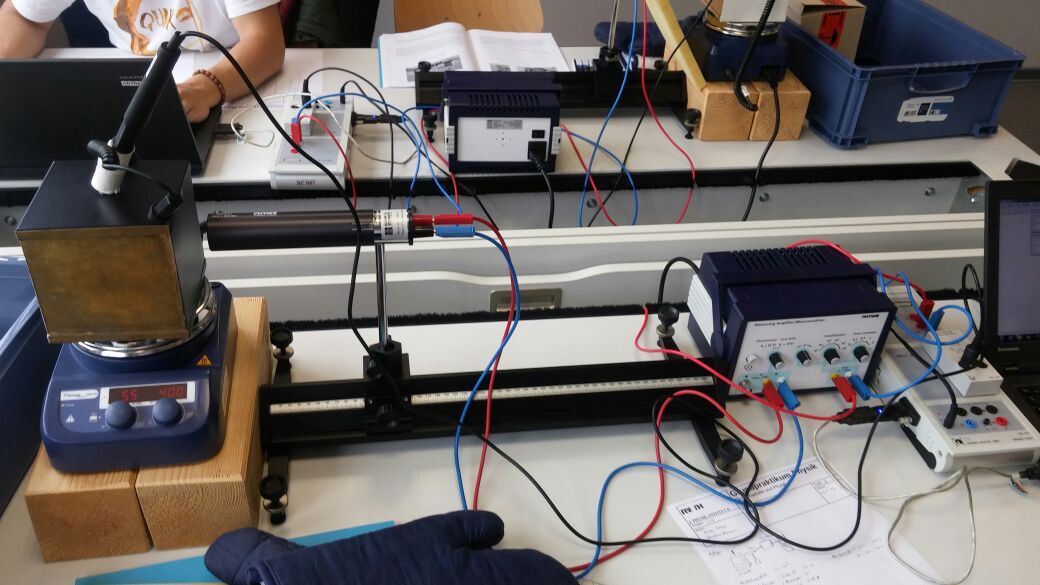
\includegraphics[scale=0.4]{Bilder/Aufbau.jpeg}
	\caption{Versuchsaufbau}
	\label{pic:Versuchsaufbau}
\end{figure}

Der Aufbau des Versuchs besteht aus einem mit Wasser gefülltem Leslie-Würfel, welcher auf einer Heizplatte erhitzt wird. Der Würfel hat vier Seiten welche alle unterschiedlich beschichtet sind. Es gibt eine verspiegelte, eine weiße, eine schwarze und eine mit Messing beschichtete Seite. In dem Lesliewürfel befindet sich ein Rührfisch, welcher von einem Magneten in der Heizplatte rotiert wird, um das warme Wasser zu verteilen und damit eine gleichmäßige Erwärmung zu gewährleisten. Durch Löcher im Deckel des Würfels werden zwei Thermometer gesteckt. Das erste Thermometer liefert die Temperatur an die Heizplatte, welche grob die Temperatur des Würfels auf den eingestellten Wert bringen bzw. halten kann. Das zweite Thermometer liefert die Temperatur an die Temperaturbox des Cassys um eine genaue Temperaturmessung des Würfels zu realisieren. Vor allem bei dem zweiten Thermometer wurde darauf geachtet, dass dieses weder den Boden noch die Wände des Würfels berührt um die genaue Temperatur des Wassers zu bestimmen.

Vor dem Würfel befindet sich außerdem eine Thermosäule nach Moll. Bei dieser wurde vorher das Schutzglas entfernt und ein Schutzrohr befestigt.
Die Thermosäule wird mit wenigen Zentimetern Abstand vor einer Seite des Würfels fest eingespannt. Als grobe Orientierung des Abstandes dient die Dicke einer Schaumstoffmatte, welche zwischen den Versuchen ebenfalls als Abschirmung der Wärmestrahlung des Würfels genutzt wird, damit sich die Thermosäule nicht über die Raumtemperatur aufheizt. Damit dies nicht geschieht wird die Säule selbst nicht angefasst um sie der Körperwärme nicht auszusetzen.

Die Thermosäule liefert zunächst eine Spannung an einen Messverstärker, welcher das Spannungssignal mit einem Faktor von $10^4$ verstärkt und die Spannung dann weiter an das Sensor-Cassy gibt.

Temperatur im Würfel sowie die Spannung der Thermosäule können nun durch das Cassy ermittelt werden.



\section{Versuchsdurchführung}

Die Thermosäule misst die Differenz der einfallenden Strahlungsleistung vom Würfel zur Strahlungsleistung durch die Umgebungstemperatur. Diese wird dann bis auf einen Konstanten Faktor, welcher für beide Gruppen (unterschiedliche Thermosäulen) unterschiedlich ist, als Spannungssignal ans Cassy weitergeleitet.

\subsection{Kalibration}
Um zu gewährleisten, dass das Spannungssignal wirklich die Leistung der Umgebungstemperatur als Referenzpunkt hat, wird die Säule auf eine Wand gerichtet und das Spannungssignal durch Offset-Einstellungen am Spannungsverstärker auf $0V$ gesetzt.

\begin{equation}
P_{gemessen}=\frac{U_{gemessen} \cdot v}{c}
\qquad
P_{theoretisch}=A_e \cdot \frac{\Omega}{\pi} \cdot \epsilon \cdot \sigma \cdot (T^4-T_0^4)
\end{equation}

Wobei der Verstärkungsvorfaktor $v=10^{-4}$ beträgt. Die Konstanten $c$ sind in Tabelle \ref{table:Empfindlichkeiten} dargestellt.

\begin{table}[h]
%\Large
\centering
	\begin{tabular}{|c|c|c|}
	\hline          & Seriennummer & Empfindlichkeit \\
	\hline Gruppe 1 & 120631 &$c_1=(0.160 \pm   0.0048)\frac{V}{W} $ \\
	\hline Gruppe 2 & 130815  &$c_2=(0.221 \pm   0.0066)\frac{V}{W} $     \\
	\hline
	\end{tabular}
\caption{Empfindlichkeiten der verwendeten Thermosäulen}
\label{table:Empfindlichkeiten}
\end{table}

Weiterhin wird eine Rauschmessung der Umgebungstemperatur sowie von Eiswasser und später siedendem Wasser durchgeführt. Die Rauschmessung der Umgebungstemperatur wird am Ende der folgenden Versuchsreihe wiederholt um sicher zu gehen, dass die Umgebungstemperatur konstant geblieben ist.
Die Messungen bei $0^\circ C$ bzw. $100^\circ C$ werden zur Temperaturkalibrierung des Thermometers benötigt.

\subsection{Messung}
Zu Beginn der Versuchsreihe wird der Würfel auf $50^\circ C$ aufgeheizt. Nun wird für jede Seite des Würfels eine Messung von circa 6 Sekunden durchgeführt, welche 125 Messwerte für Temperatur im Würfel und Spannung an der Thermosäule aufnimmt.
Wurde dies für alle 4 verschiedenen Seiten durchgeführt, erhitzt man den Würfel um $5^\circ C$ und wiederholt die 4 Messungen. Dieser Vorgang wird bis zur einer Endtemperatur von $95^\circ C$ wiederholt.
Die genauen Einstellungen bei den Messungen mit dem Sensor-Cassy sind in Tabelle \ref{table:Einstellungen} dargestellt.
 
\begin{table}[h]
\centering
	\begin{tabular}{|c|c|c|c|}
	\hline Messintervall & Messwertanzahl & Messzeit & Spannungsmessbereich \\
	\hline $50ms$& 125& $6.25s$& $-10V...+10V$ \\
	\hline
	\end{tabular}
\caption{Einstellungen am Cassy}
\label{table:Einstellungen}
\end{table}

Der Spannungsmessbereich wurde nur bei der Gruppe 2 bei der schwarzen und weißen Seite des Würfels ab $70^\circ C$ auf $-30V$ bis $30 V$ erhöht, wobei für $70^\circ C$ und $75^\circ C$ beide Bereichswerte gemessen wurden um zu überprüfen welche Auswirkung die Änderung des Spannungsmessbereich auf die Werte hat.


\newpage
\section{Auswertung}
\subsection{Kalibration}
Zunächst wurde die Kalibrierung der Temperatur durchgeführt. Aus den beiden Rauschmessungen erhalten Mittelwerte, dargestellt in Tabelle \ref{table:Kalibrationsmessungen}.

\begin{table}[h]
\centering
	\begin{tabular}{|c|c|c|}
	\hline Gruppe1 & $T_{100^\circ}= (371.079 \pm 0.006)  K$ & $T_{0^\circ}=  (274.453 \pm 0.009) K$\\
	\hline Gruppe2 & $T_{100^\circ}=  (370.936 \pm 0.011) K$ & $T_{0^\circ}=(274.672 \pm 0.06)   K$\\
	\hline
	\end{tabular}
\caption{Kalibrationsmessungen (gemittelt) beider Gruppen}
\label{table:Kalibrationsmessungen}
\end{table}

\begin{figure}[H]
	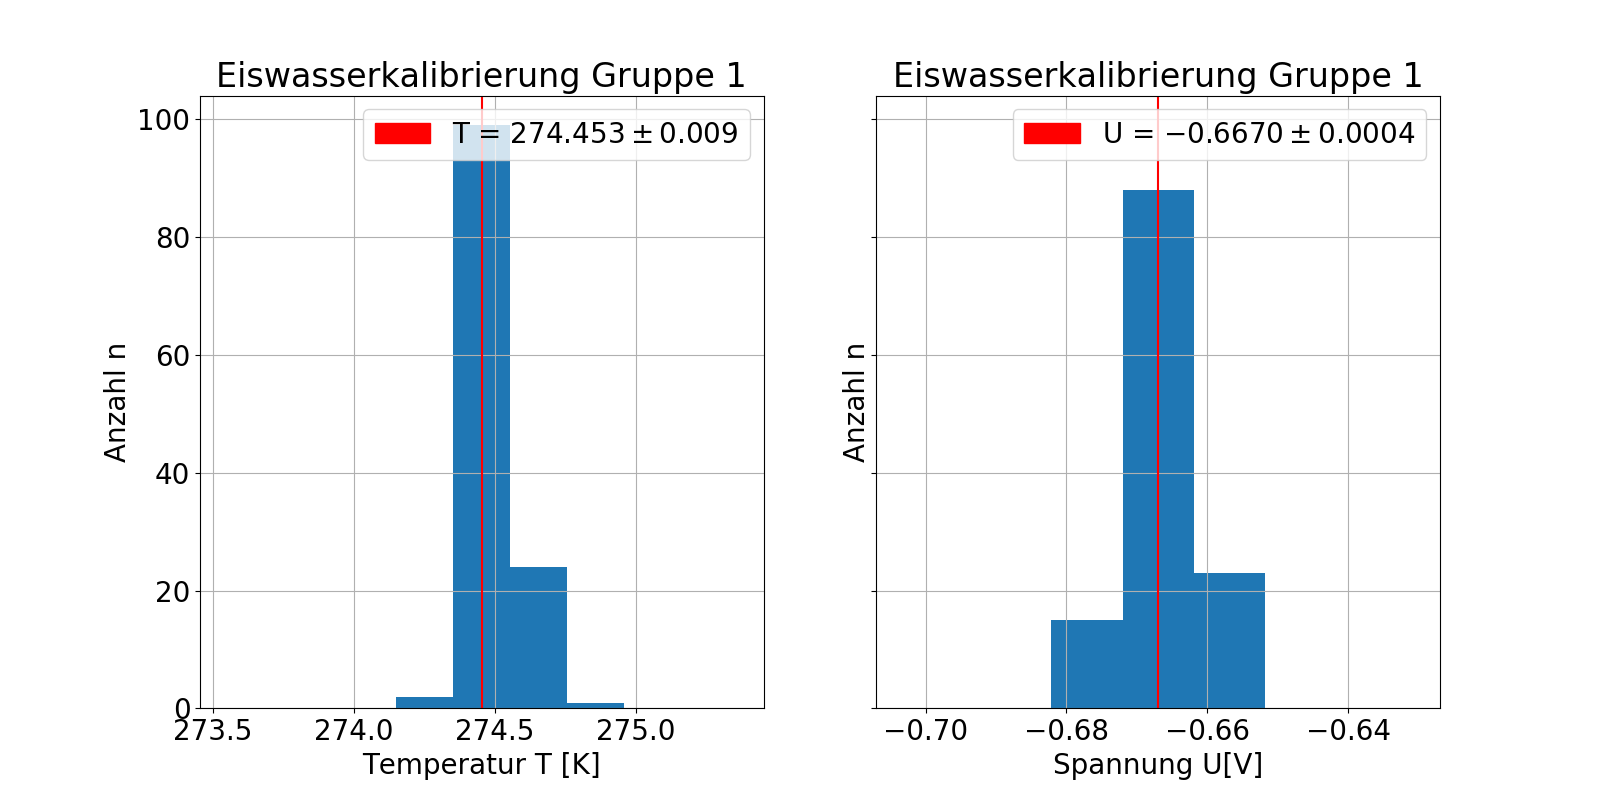
\includegraphics[scale=0.4]{Bilder/Gruppe1_Eiswasser.png}%
	\caption[Gruppe 1 Eiswassermessung]{Gruppe 1 Eiswassermessung}%
	\label{pic:G1Eismessung}%
\end{figure}

\begin{figure}[H]
	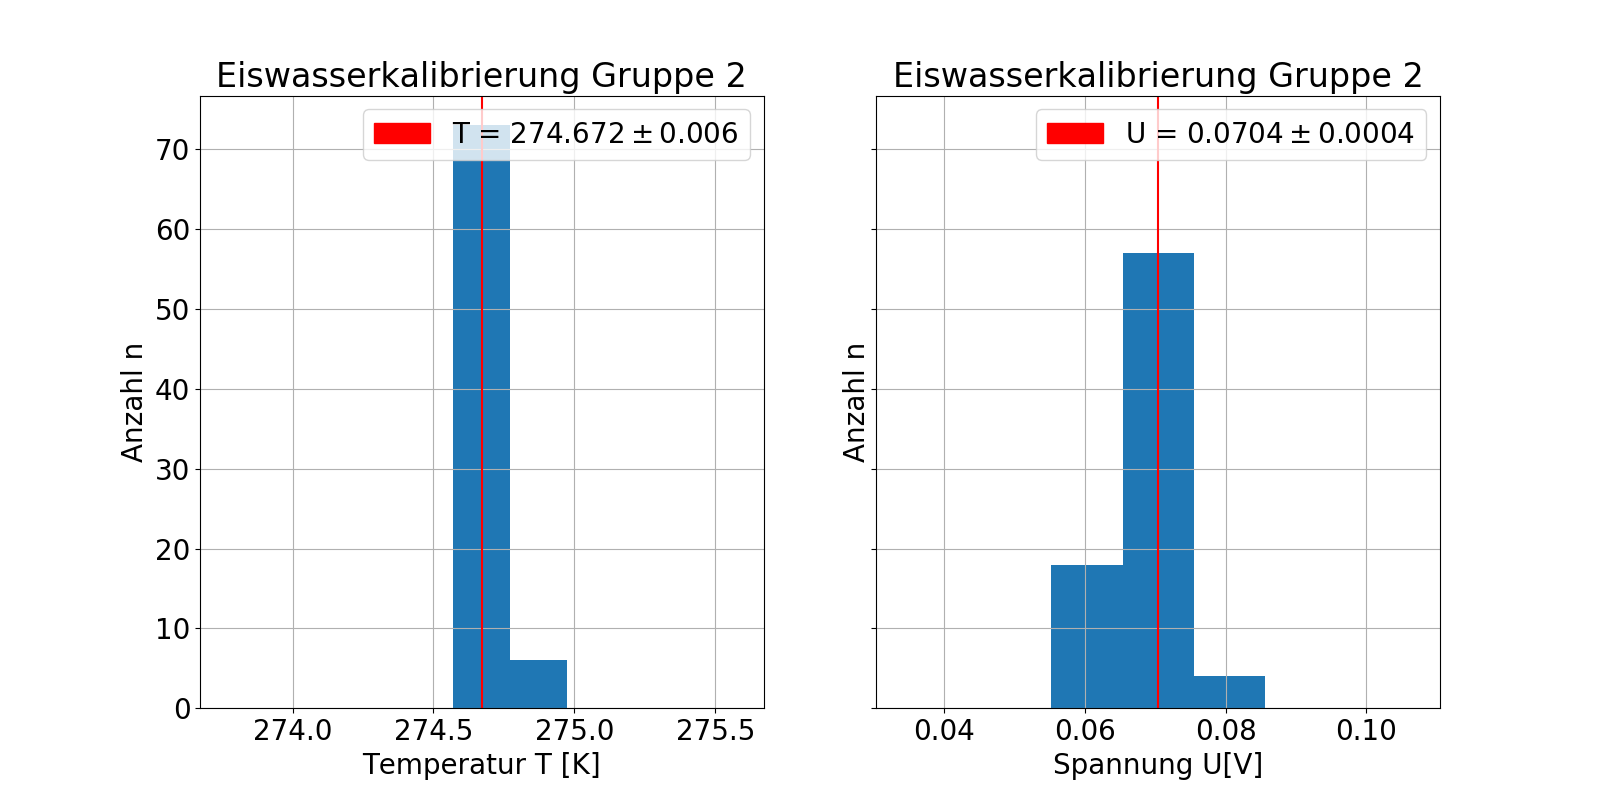
\includegraphics[scale=0.4]{Bilder/Gruppe2_Eiswasser.png}%
	\caption[Gruppe 2 Eiswassermessung]{Gruppe 2 Eiswassermessung}%
	\label{pic:G2Eismessung}%
\end{figure}

\begin{figure}[H]
	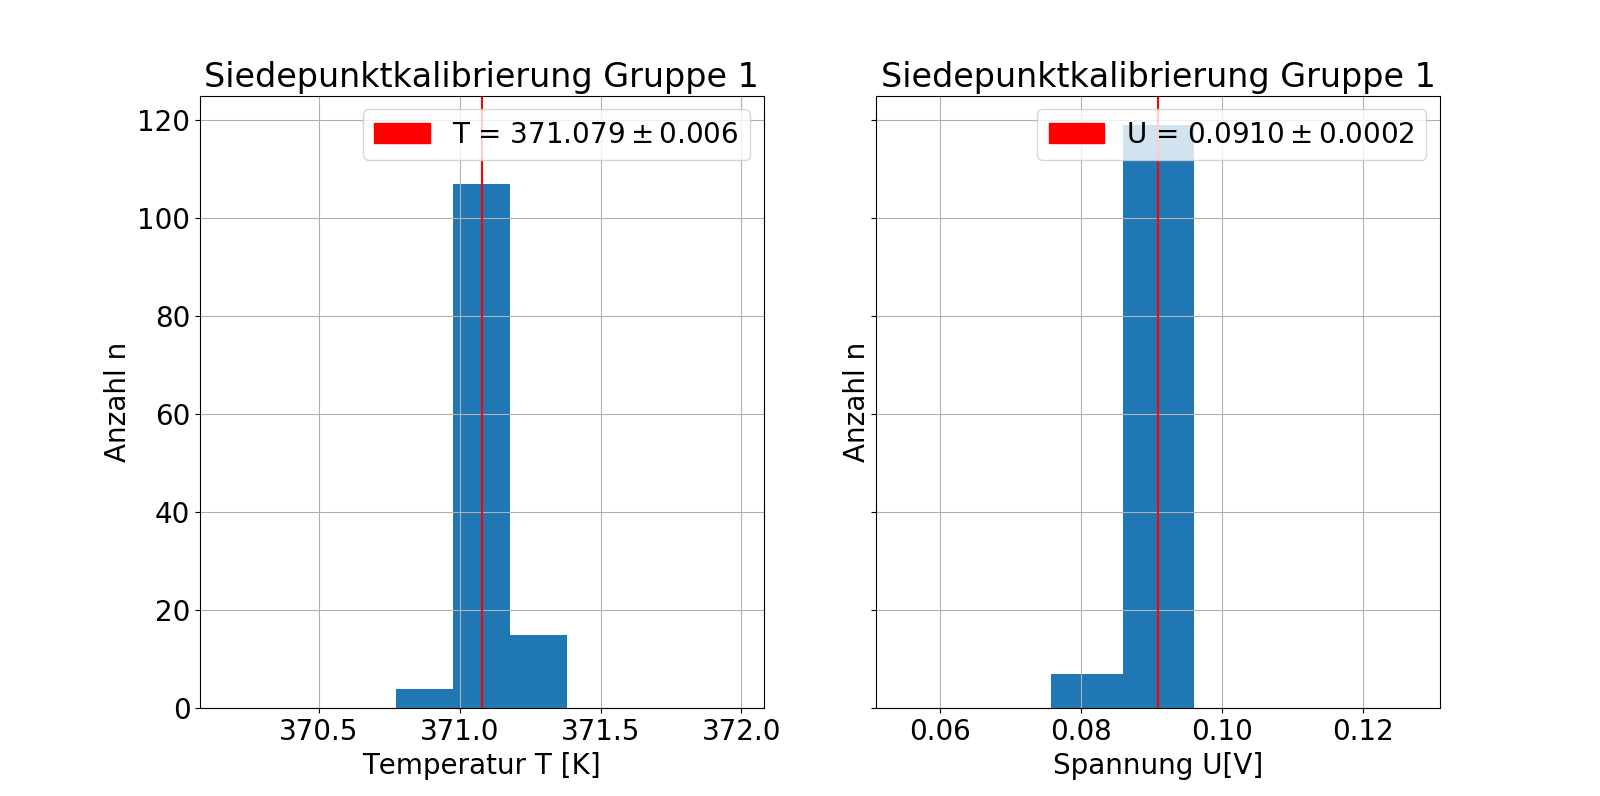
\includegraphics[scale=0.4]{Bilder/Gruppe1_kochendesWasser.png}%
	\caption[Gruppe 1 Siedemessung]{Gruppe 1 Siedemessung}%
	\label{pic:G1Siedemessung}%
\end{figure}

\begin{figure}[H]
	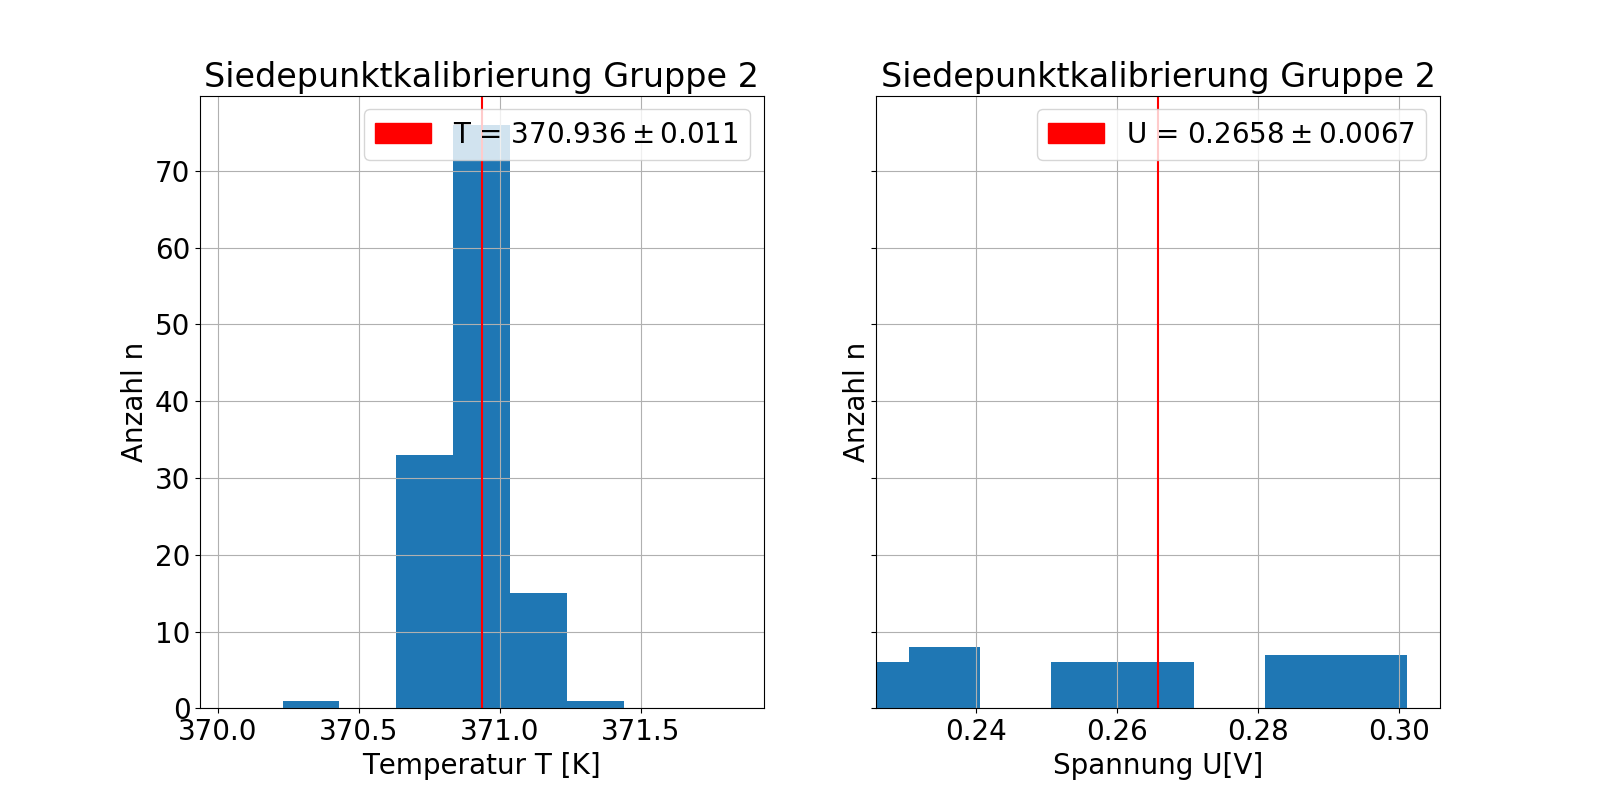
\includegraphics[scale=0.4]{Bilder/Gruppe2_kochendesWasser.png}%
	\caption[Gruppe 2 Siedemessung]{Gruppe 2 Siedemessung}%
	\label{pic:G12Siedemessung}%
\end{figure}


Um mit Hilfe der Kalibration die realen Temperaturen aus den Gemessenen zu berechnen definieren wir
\begin{eqnarray*}
\qquad T_{real} = m \cdot T_{gemessen} + n \qquad	\\
m = \frac{273.15K}{T_{100^\circ} - T_{0^\circ}}
\qquad
n = 273.15K - m \cdot T_{0^\circ}
\end{eqnarray*}

Mit dieser Formel wurden nun alle Messwerte der anderen Messungen kalibriert und die Auswertung mit $T_{real}$ weitergeführt.

\begin{table}[H]
\centering
	\begin{tabular}{|c|c|c|}
	\hline Gruppe 1 & $m = 1.035$ & $n =-10.89 K$\\
	\hline Gruppe 2 & $m = 1.039 $ & $n = -12.181 K$\\
	\hline
	\end{tabular}
\caption{Kalibrationsergebnisse für $T_{real} = m \cdot T_{gemessen}+b$}
\label{table:KalibrationTreal}
\end{table}

Die kalibrierten Werte für die Raumtemperatur $T_0$ sind in Tabelle \ref{table:KalibrationT0} dargestellt.

\begin{table}[h]
\centering
	\begin{tabular}{|c|c|}
	\hline Gruppe 1& Gruppe 2\\
	\hline $T_0= (297.501 \pm 0.005) K$ & $T_0= (298.053 \pm 0.006)   K$\\
	\hline
	\end{tabular}
\caption{Kalibrationsergebnisse für Raumtemperatur $T_0$}
\label{table:KalibrationT0}
\end{table}

\subsection{Lineare Regression an $T^4$}

Nun wird eine lineare Regression der Spannung $U(T)$ über $T^4-T_0^4$ für jede Seite beider Würfel durchgeführt.
\begin{equation}
U(T) = a \cdot (T^4-T_0^4)+b
\end{equation} 

Dafür werden Mittelwerte und Standartabweichung von $U,T$ und $T_0$ aus den 125 kalibrierten Messwerten jeder Messung berechnet und für die lineare Regression verwendet.
Da wir also Fehler auf $x$ und $y$ Werte haben, benutzen wir die zur Verfügung gestellte Praktikumsroutine \texttt{lineare\_regression\_xy()}. 
Die Fehler auf die x Werte berechnen sich wie folgt:

\begin{equation}
x=T^4-T_0^4
\qquad
\sigma_x = \sqrt{(4 \cdot T^3 \cdot\sigma_T)^2+(4\cdot T_0^3\cdot \sigma_{T_0})^2} 
\end{equation}

Aus der linearen Regression bekommen wir Werte und Fehler für $a$ und $b$ für jede Seite \ref{table:ErgebnisseLinregress}.
Beispielhaft ist das Ergebnis der linearen Regression für die weiße Seite des Leslie-Würfels bei Gruppe in Abbildung \ref{pic:LinregressG1weiss} dargestellt.

\begin{table}[H]
\Large
\centering
	\begin{tabular}{|c|c|c|}
	\hline Seite & Gruppe 1& Gruppe 2 \\
	\hline Schwarz& $a=( 0.895\pm 0.008)\cdot 10^{-9}\frac{V}{K^4} $ &  $a=( 1.373\pm 0.017 )\cdot 10^{-9}\frac{V}{K^4}$\\
	         $ $  & $b=(-0.21 \pm 0.06)V $ &  $b=( 0.03\pm 0.11)V $\\
	$ $  & $\frac{\chi^2}{ndof}=126$ &  $\frac{\chi^2}{ndof}=317$\\
	\hline Weiß& $a=( 0.856\pm 0.006)\cdot 10^{-9}\frac{V}{K^4} $ &  $a=(1.318 \pm 0.023)\cdot 10^{-9}\frac{V}{K^4}$\\
	     $ $       & $b=(-0.06 \pm 0.04)V $ &  $b=(0.15\pm 0.15)V $\\
	$ $  & $\frac{\chi^2}{ndof}=78$ &  $\frac{\chi^2}{ndof}=525$\\
	\hline Messing& $a=(0.062 \pm 0.005)\cdot 10^{-9}\frac{V}{K^4} $ &  $a=( 0.097\pm 0.003)\cdot 10^{-9}\frac{V}{K^4}$\\
	     $ $       & $b=(0.05 \pm 0.03)V $ &  $b=(0.149 \pm 0.023)V $\\
	$ $  & $\frac{\chi^2}{ndof}=2714$ &  $\frac{\chi^2}{ndof}=2626$\\
	\hline Spiegel& $a=(0.0396 \pm 0.0018)\cdot 10^{-9}\frac{V}{K^4} $ &  $a=(0.061\pm 0.003 )\cdot 10^{-9}\frac{V}{K^4}$\\
	     $ $       & $b=(0.105 \pm 0.011)V $ &  $b=(0.132 \pm 0.025 )V $\\
	$ $  & $\frac{\chi^2}{ndof}=842$ &  $\frac{\chi^2}{ndof}=5190$\\
	           
	
	\hline  
	
	\end{tabular}
\caption{Ergebnisse der linearen Regression}
\label{table:ErgebnisseLinregress}
\end{table} 

\begin{figure}[H]
	\centering
	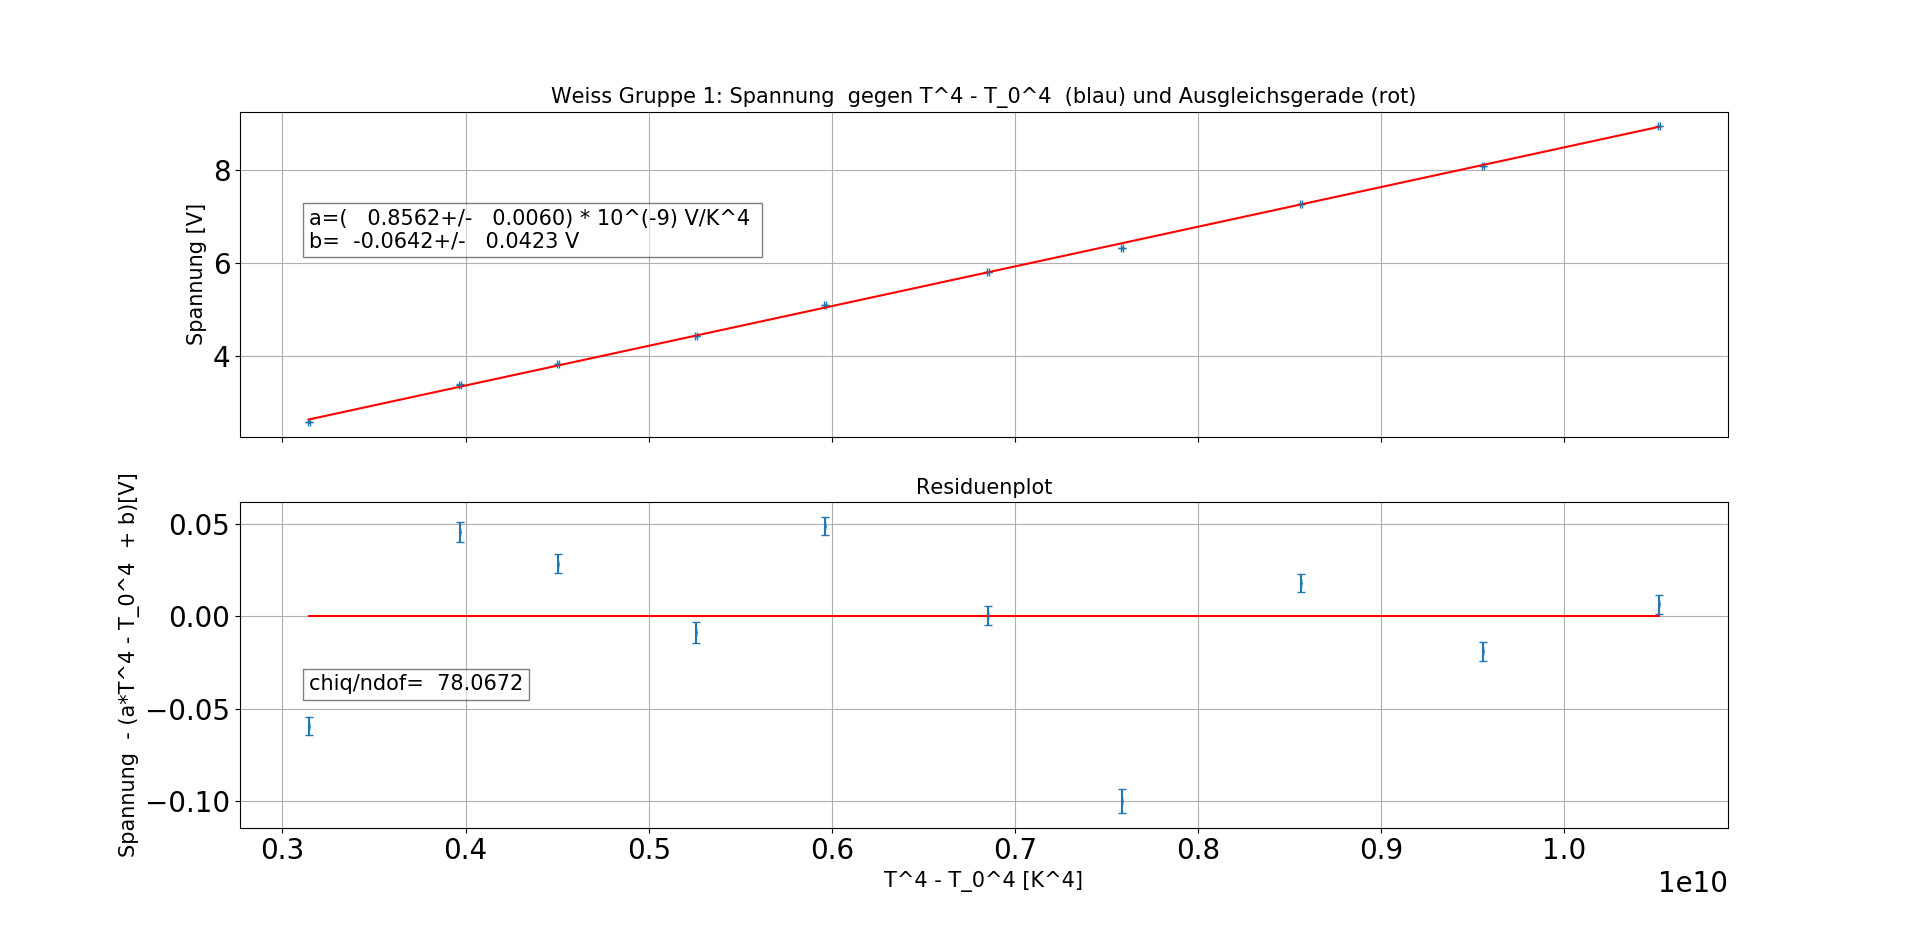
\includegraphics[scale=0.35]{Bilder/Gruppe1_Weiss.png}%
	\caption{lineare Regression der Gruppe 1, weiße Seite}%
	\label{pic:LinregressG1weiss}%
\end{figure}


\subsection{Bestimmung der Emissionskoeffizienten}

Wir können mit den im Theorieteil hergeleiteten Formeln \ref{eq:epsilon} nun die Emissionskoeffizienten einer Seite leicht aus der Steigung bestimmen.
\begin{equation}
\epsilon = \frac{\frac{U \cdot v}{c}}{P_{ideal}} = a \cdot \frac{\pi \cdot r^2 \cdot v}{A_s \cdot A_e \cdot \sigma \cdot c}
\end{equation}

Die Fehler auf den Emissionskoeffizient ergeben sich aus:
\begin{equation}
\sigma_{\epsilon,stat}=\frac{v r^2 \pi}{A_s A_e \sigma c}\cdot  \sigma_a \qquad
\sigma_{\epsilon ,sys}=\frac{a v r^2 \pi}{A_sA_e \sigma c^2}\cdot \sigma_c
\end{equation}

Daraus berechnen sich die in Tabelle \ref{table:Epsilon} durch $\epsilon \pm \sigma_{stat}\pm \sigma_{sys} $ dargestellten Ergebnisse.
\begin{table}[H]
\Large
\centering
	\begin{tabular}{|c|c|c|}
	\hline Seite & Gruppe 1& Gruppe 2 \\
	\hline Schwarz& $\epsilon=0.905 \pm 0.008\pm 0.027$ &  $\epsilon=1.004 \pm  0.012 \pm 0.03 $\\
	\hline Weiß & $\epsilon=0.865 \pm 0.006\pm 0.03$ & $\epsilon= 0.964\pm 0.016 \pm 0.029$\\
	\hline Messing & $\epsilon=0.0627 \pm 0.0048\pm 0.0019$ & $\epsilon=0.0706 \pm 0.0023\pm 0.0021$\\
	\hline Spiegel & $\epsilon=0.0400 \pm 0.0018\pm 0.0012$ & $\epsilon=0.0449 \pm 0.0024\pm 0.0013$\\
	\hline  
	\end{tabular}
\caption{Ergebnisse für $\epsilon$ mit statistischen und systematischen Fehlern}
\label{table:Epsilon}
\end{table}

Um die Ergebnisse der beiden Gruppen besser vergleichen zu können werden die Quotienten der Emissionskoeffizienten zur jeweiligen schwarzen Seite gebildet.
\begin{equation}
\epsilon_{rel}=\frac{\epsilon_i}{\epsilon_{Schwarz}} 
\qquad
\sigma_{\epsilon_{rel}}=\sqrt{\left(\frac{\epsilon_i}{\epsilon_{Schwarz}^2} \cdot  \sigma_{\epsilon,Schwarz}\right) ^2 + \left( \frac{1}{\epsilon_{Schwarz}}\cdot \sigma_{\epsilon,i}\right) ^2}
\end{equation}

Daraus folgen folgende Relativwerte in Tabelle \ref{table:EpsilonRel}.
\begin{table}[H]
\centering
	\begin{tabular}{|c|c|c|}
	\hline Relativwerte zu Schwarz von & Gruppe 1 & Gruppe 2\\
	\hline Weiß & $\epsilon_{rel}=0.956 \pm 0.011 \pm 0.041 $ & $\epsilon_{rel}=0.960 \pm 0.02\pm 0.04$\\
	\hline Messing & $\epsilon_{rel}=0.069 \pm 0.009 \pm 0.030$ & $\epsilon_{rel}= 0.070\pm 0.012 \pm 0.030$\\
	\hline Spiegel & $\epsilon_{rel}=0.044 \pm 0.009 \pm 0.030$ & $\epsilon_{rel}= 0.045\pm 0.012 \pm 0.030$\\
	\hline  
	\end{tabular}
\caption{Relativwerte der Emissionskoeffizienten}
\label{table:EpsilonRel}
\end{table}

\subsection{Fit an $T^x$}
Zum Schluss wird noch ein weiterer Fit gemacht, durch den die 4-rer Potenz der Temperatur im \textit{Stefan-Boltzmann Gesetz} \ref{eq:SBG} überprüft werden soll.
Dafür fitten wir $U$ an $T^{p_2}$ mit den Fitparametern $p_0,p_1$ und $p_2$.
\begin{equation}
U(T) = p_0 + p_1 \cdot T^{p_2}
\end{equation}
Hierbei ist die Referenz zu $T_0$ in dem Parameter $p_0$ einbezogen.
Für den Fit benutzen wir die Funktion \texttt{scipy.optimize.curvefit()}, welche ohne Fehler arbeitet\footnote{Die Funktion gibt zwar Fehler aus, wenn man jedoch Fehler auf die Werte übergibt, konvergiert die Routine nicht}.
Dabei wurden die Anfangswerte zu $p_0$ und $p_1$ aus den vorher bestimmten Steigungen und Achsenabschnitten der linearen Regressionen gewählt.
\begin{equation*}
p_0=b-a\cdot T^4 \qquad p_1=a
\end{equation*}
Bei dieser Auswertung konvergieren nur zwei Anpassungen. Bei der ersten Gruppe konvergieren die Werte der weißen Seite und bei der zweiten Gruppe die der Messing-Seite, zu sehen in Tabelle \ref{table:ErgebnisseTxFit} :

\begin{table}[H]
\Large
\centering
	\begin{tabular}{|c|c|c|c|}
	\hline $ U=p_0+p_1\cdot T^{p_2}$& $p_0$& $p_1$ & $p_2$\\
	\hline Gruppe 1 / Weiß & $(-7.0 \pm 1.5)V $ & $ (1.5 \pm 4.4  )\cdot 10^{-9}\frac{V}{K^4}$  & $ 3.9\pm 0.5 $ \\
	\hline Gruppe 2 / Messing &  $(-0.7 \pm 0.7)V $ & $ (0.4 \pm 4.3  )\cdot 10^{-9}\frac{V}{K^4}$  & $ 3.8\pm 1.9 $  \\
	\hline
	\end{tabular}
\caption{Ergebnisse der Fitparameter für $T^x$-Anpassung}
\label{table:ErgebnisseTxFit}
\end{table}

\newpage

\begin{figure}[H]
	\hskip -2 cm
	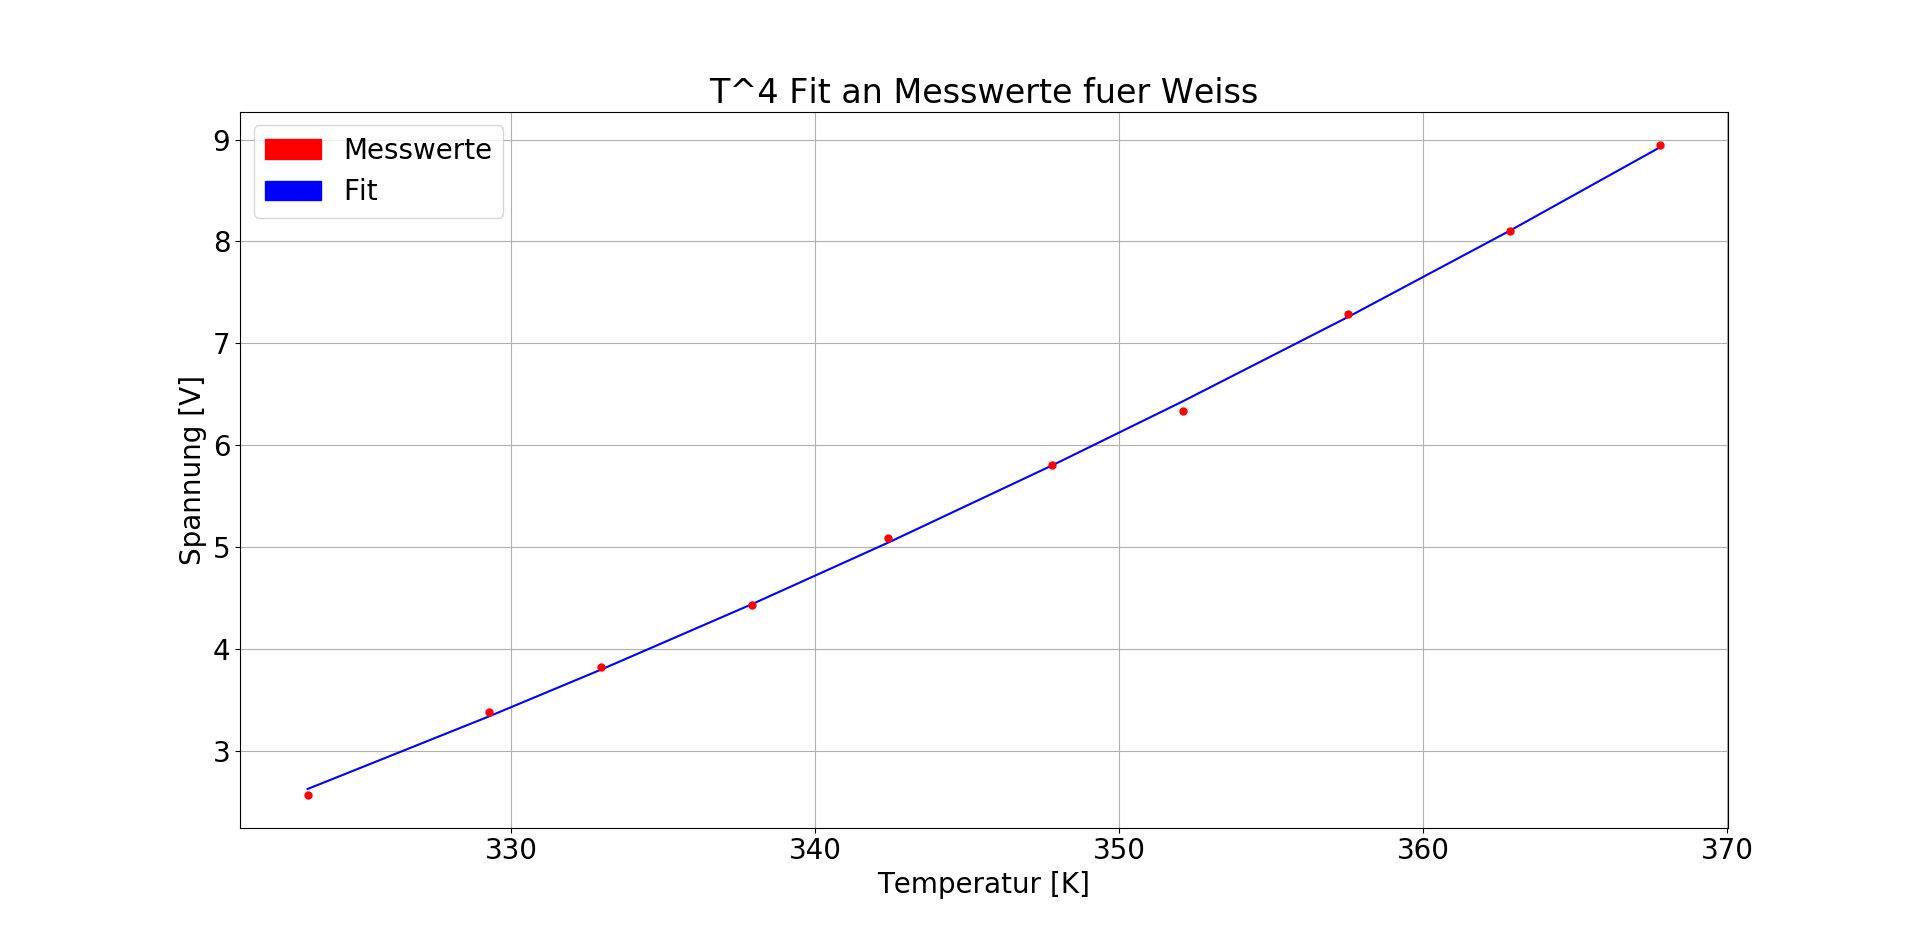
\includegraphics[scale=0.42]{Bilder/Gruppe1_Fit_Weiss.png}%
	\caption{$T^x$-Fit für die 1. Gruppe zur weißen Seite}%
	\label{pic:T4FitG1Weiss}%
\end{figure}

\begin{figure}[H]
	\hskip -2 cm
	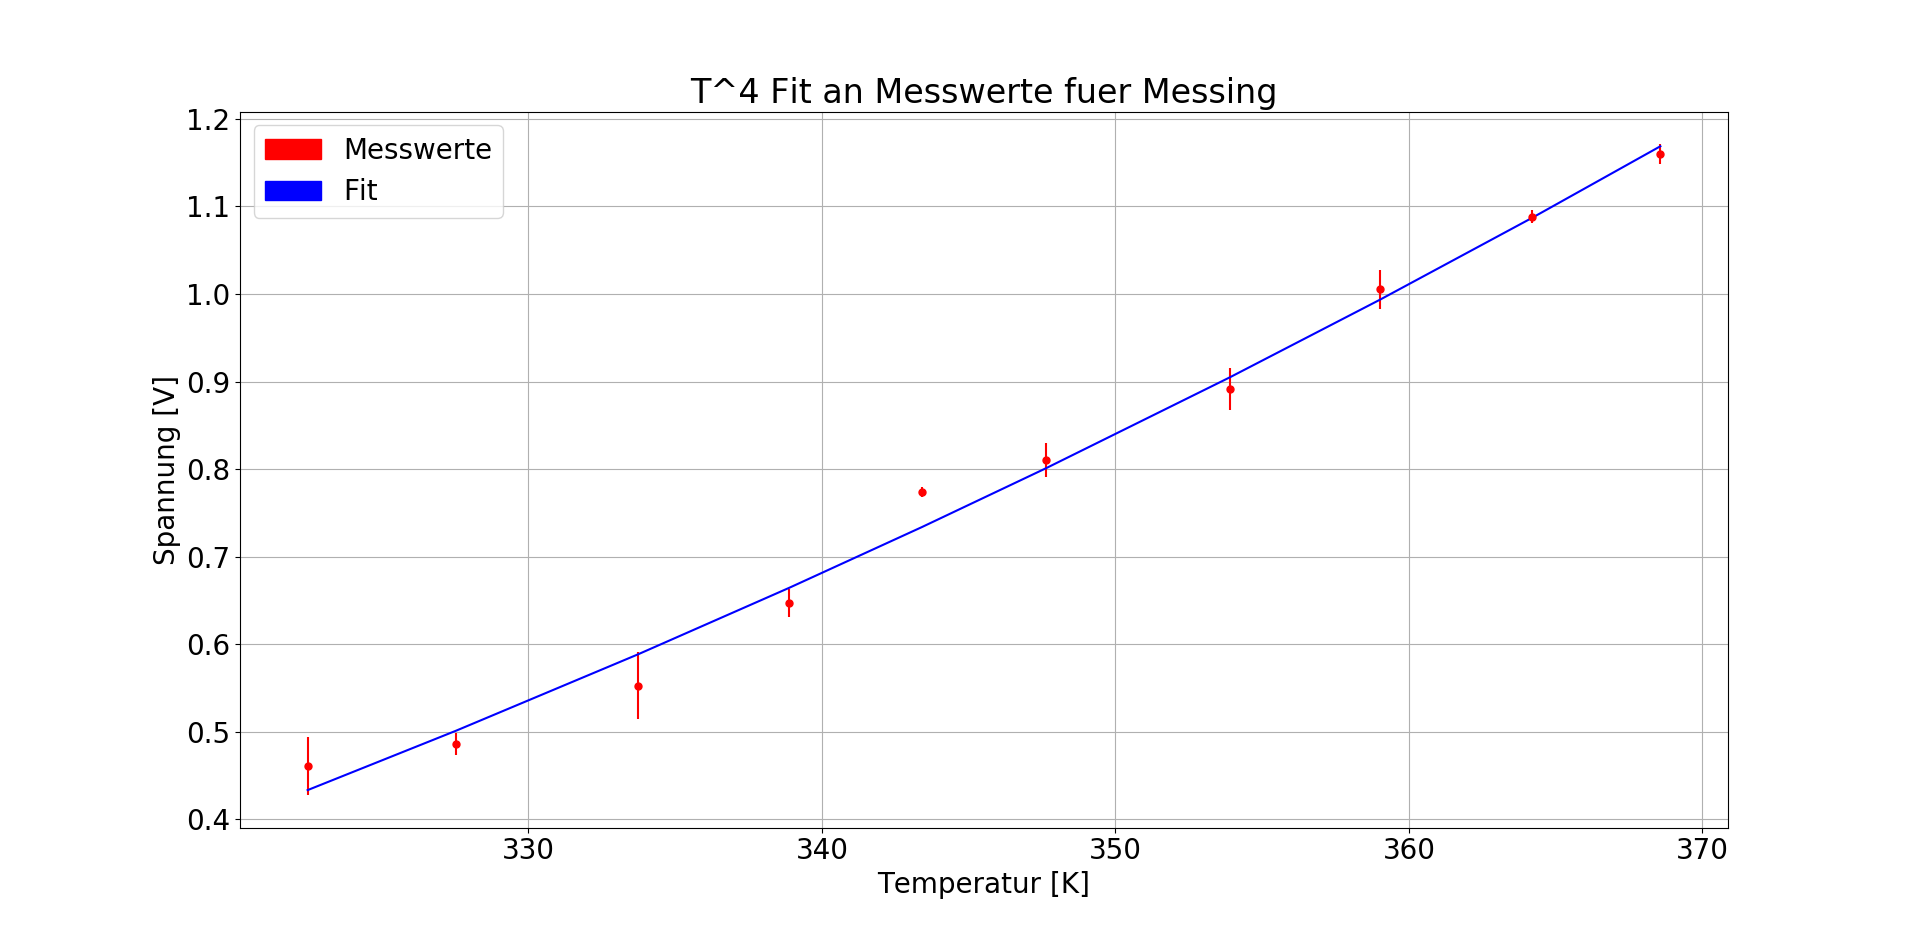
\includegraphics[scale=0.42]{Bilder/Gruppe2_Fit_Messing.png}%
	\caption{$T^x$-Fit für die 2. Gruppe zur Messing-Seite}%
	\label{pic:T4FitG2Messing}%
\end{figure}

\newpage
\section{Fazit}

Zunächst einmal ist auffällig, dass die $\frac{\chi^2}{ndof}$ bei den linearen Regressionen sehr groß sind. Außerdem sind die Werte für die Emissionskoeffizienten unrealistisch, da z.B. der Wert der zweiten Gruppe für die schwarze Seite über 1 liegt und damit unphysikalisch ist. Außerdem erwarten wir bei der weißen Seite dieser Gruppe einen nicht ganz so nah an 1 liegenden Wert.

Dies Auffälligkeiten könnten durch nicht berücksichtigte Fehler entstanden sein. Jedoch ist wahrscheinlich, dass die Empfindlichkeitsangaben der Thermosäule nicht sehr präzise sind. Denn diese Konstante fällt raus wenn wir uns die relativen Emissionskoeffizienten zur schwarzen Seite anschauen, da diese eine Abweichung von unter einer Standartabweichung haben.

Somit können wir festhalten, dass die diskrete Bestimmung der Emissionskoeffizienten aufgrund ungenauer Angaben der Empfindlichkeit nicht perfekt geklappt hat, aber die Messungen selbst erfolgreich waren, da sich bei den beiden Gruppen ähnliche Werte für die relativen Emissionskoeffizienten ergeben haben.

Die Auswertung durch den Fit an einen freien Exponenten für T war zwar durch Konvergenzprobleme in der Pythonroutine \texttt{scipy.optimize.curvefit()}  nur bei 2 Messreihen erfolgreich, jedoch ist der Exponent durch die erreichten Werte angemessen bestätigt, da der Wert 4 innerhalb von einer Standartabweichung vom bestimmten Wert liegt (siehe Tabelle \ref{table:ErgebnisseTxFit}).

\newpage
\section{Anhang}

\begin{center}

\begin{figure}[H]
	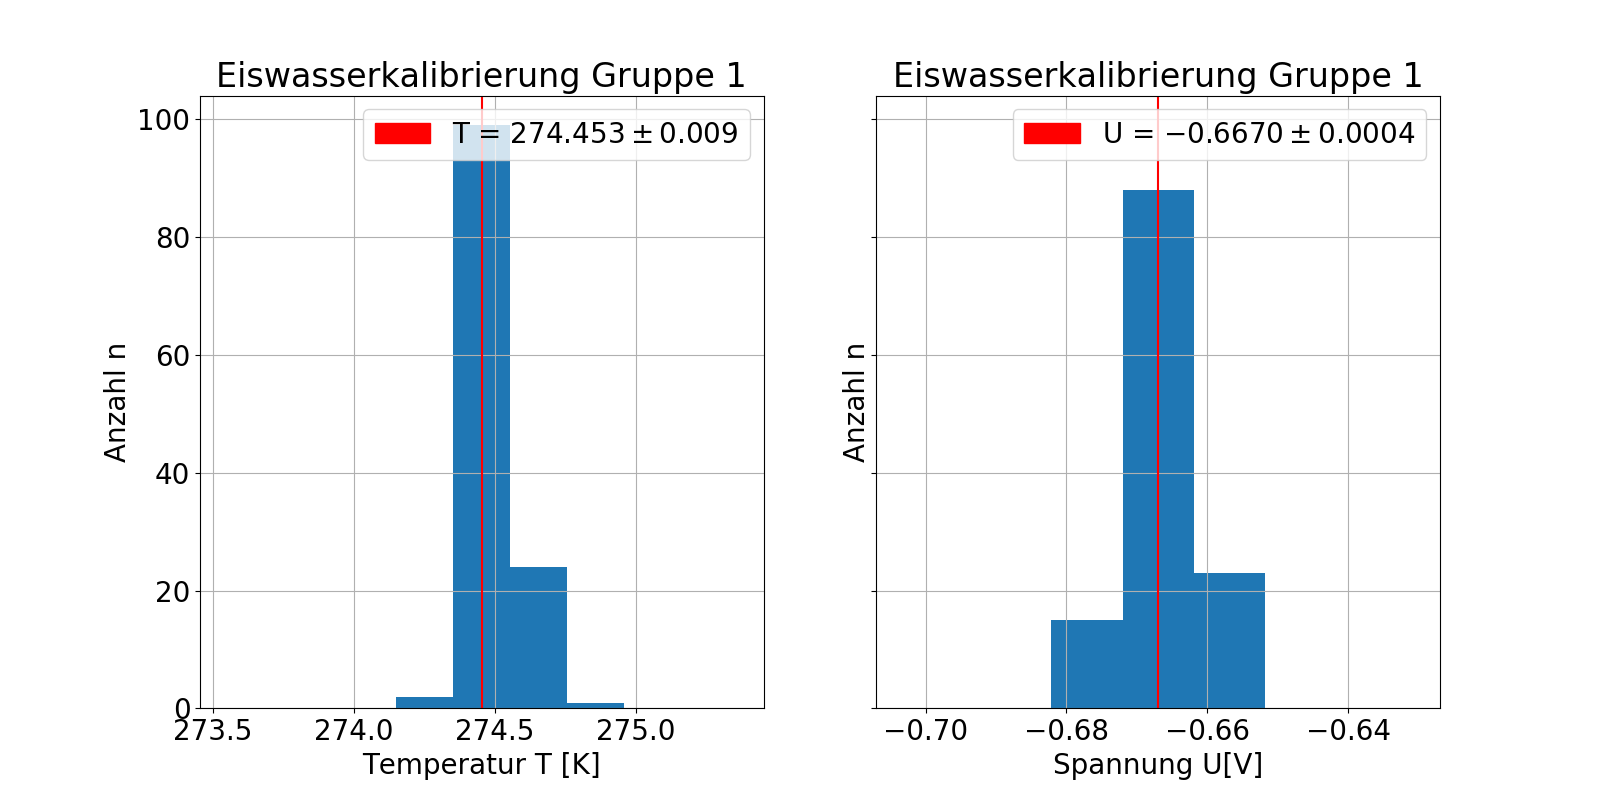
\includegraphics[scale=0.4]{Bilder/Gruppe1_Eiswasser.png}%
	\caption[Gruppe 1 Eiswassermessung]{Gruppe 1 Eiswassermessung}%
	\label{pic:Abbildung 2}%
\end{figure}

\begin{figure}[H]
	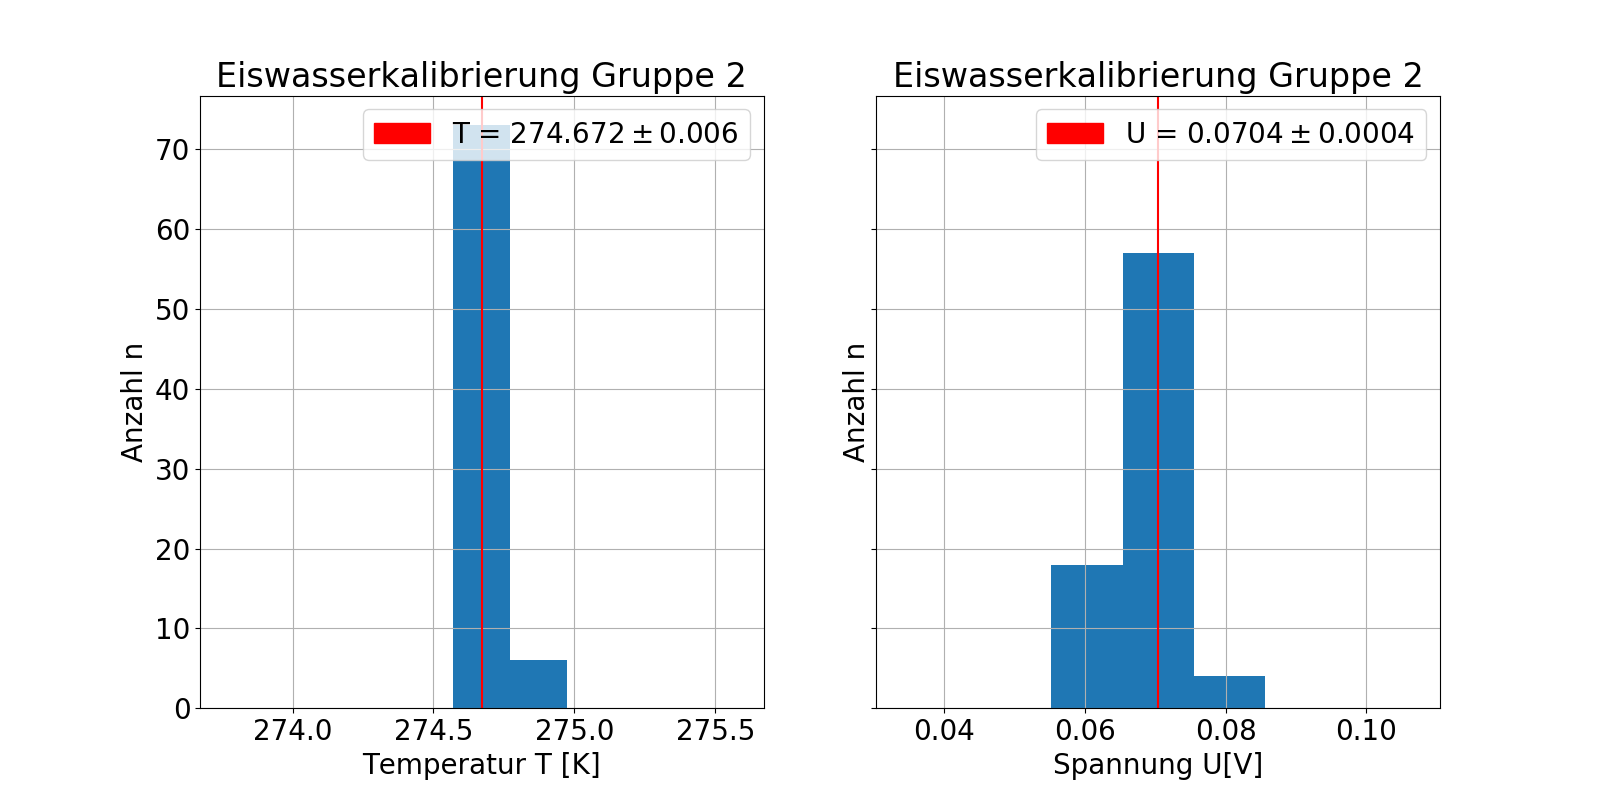
\includegraphics[scale=0.4]{Bilder/Gruppe2_Eiswasser.png}%
	\caption[Gruppe 2 Eiswassermessung]{Gruppe 2 Eiswassermessung}%
	\label{pic:Abbildung 2}%
\end{figure}

\begin{figure}[H]
	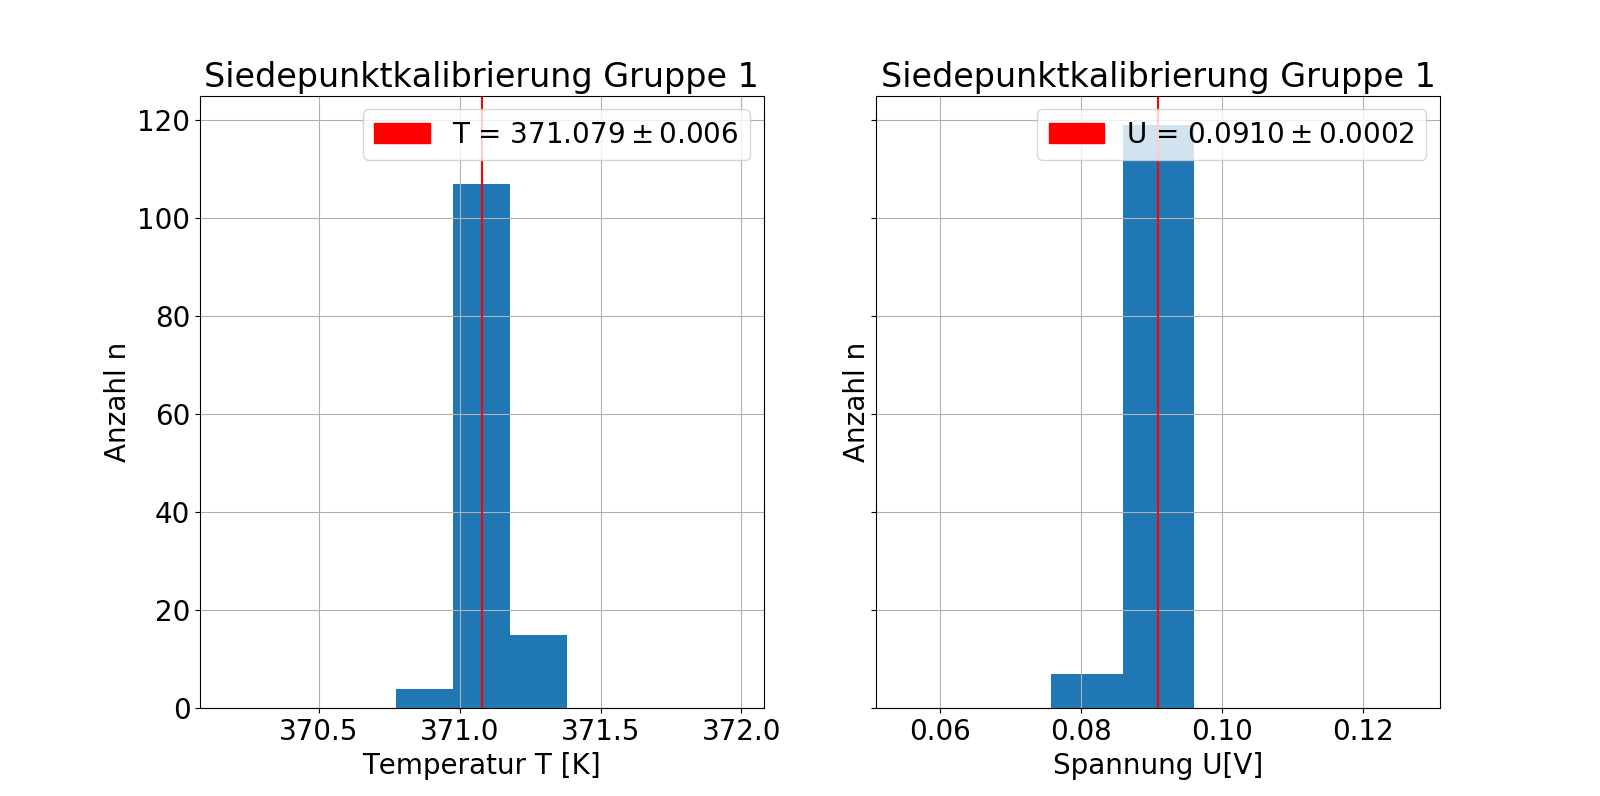
\includegraphics[scale=0.4]{Bilder/Gruppe1_kochendesWasser.png}%
	\caption[Gruppe 1 Siedemessung]{Gruppe 1 Siedemessung}%
	\label{pic:Abbildung 2}%
\end{figure}

\begin{figure}[H]
	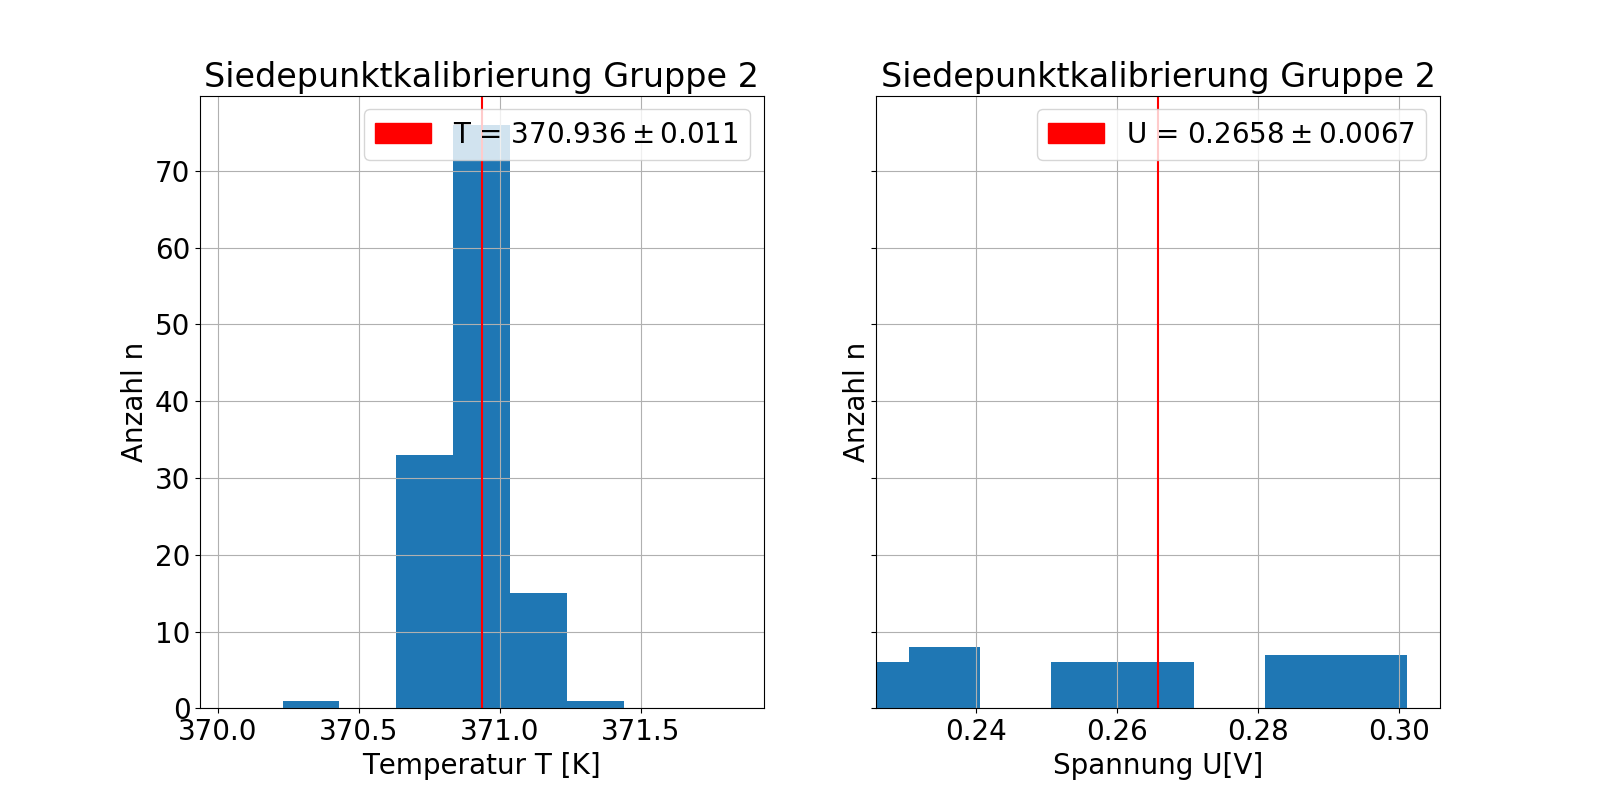
\includegraphics[scale=0.4]{Bilder/Gruppe2_kochendesWasser.png}%
	\caption[Gruppe 2 Siedemessung]{Gruppe 2 Siedemessung}%
	\label{pic:Abbildung 2}%
\end{figure}

\begin{figure}[H]
	\hskip -2 cm
	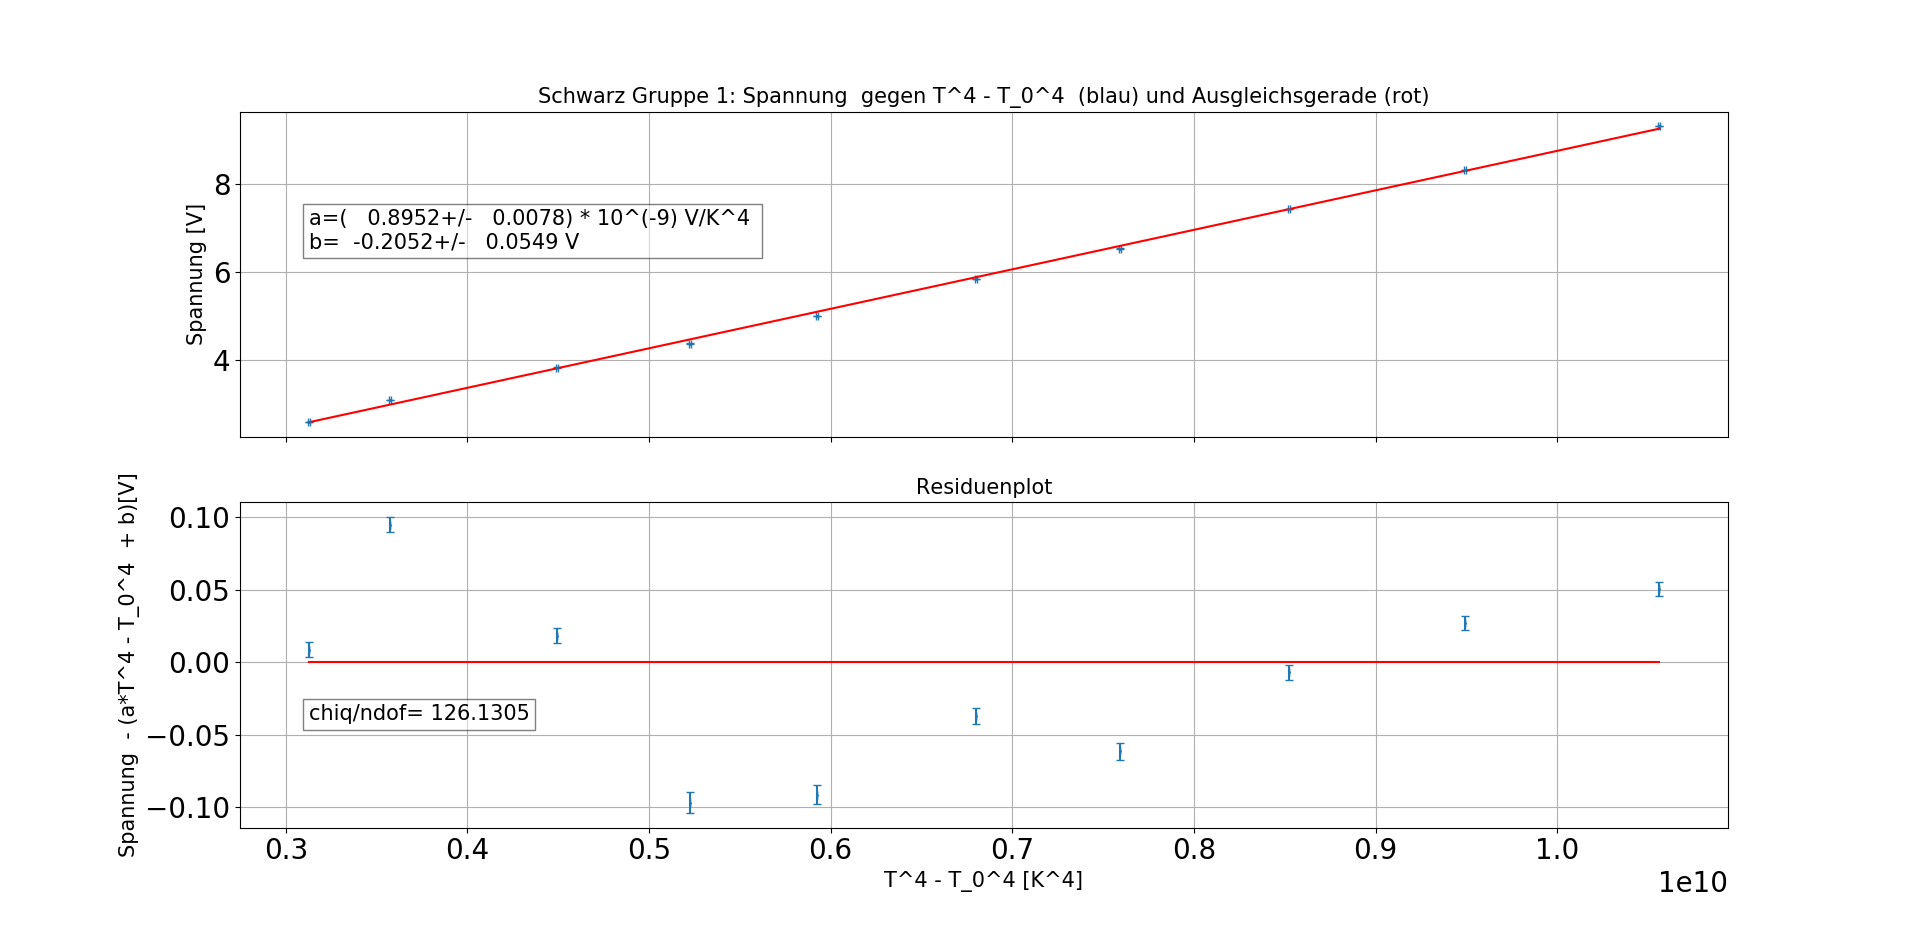
\includegraphics[scale=0.42]{Bilder/Gruppe1_Schwarz.png}%
	\caption[lineare Regression für die 1 Gruppe zur schwarzen Seite]{lineare Regression für die 1 Gruppe zur schwarzen Seite}%
	\label{pic:Abbildung 2}%
	
\end{figure}

\begin{figure}[H]
	\hskip -2 cm
	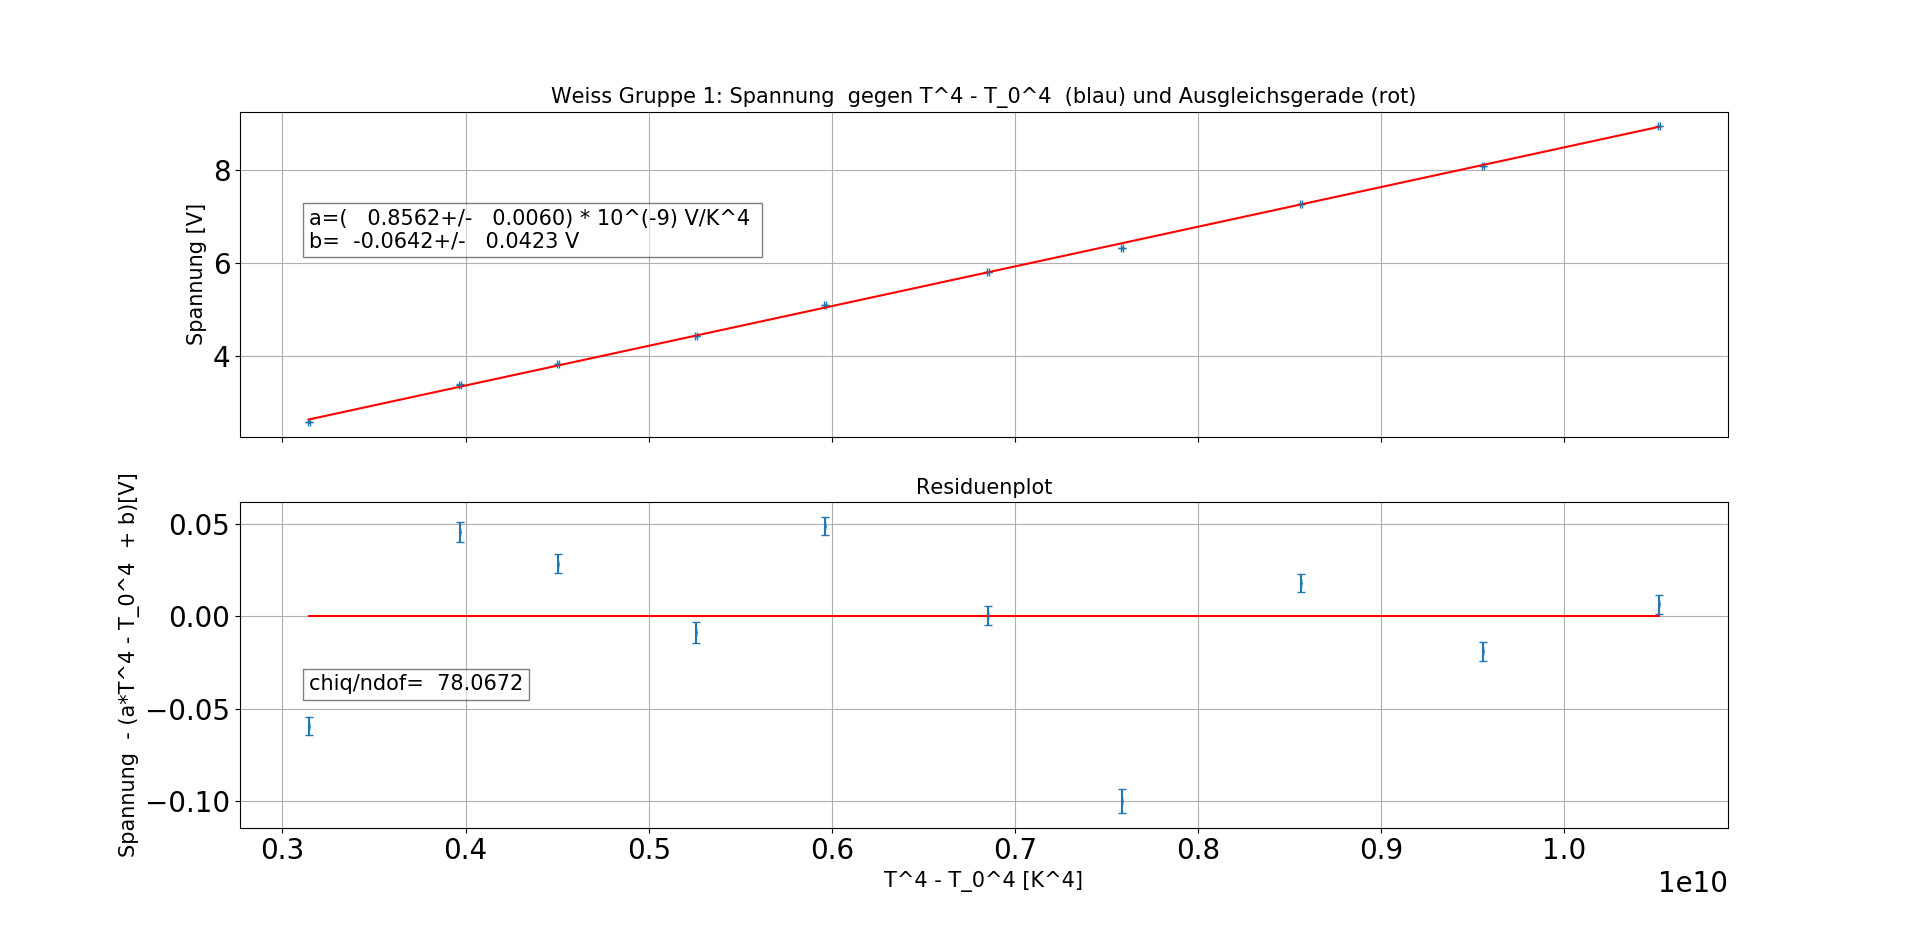
\includegraphics[scale=0.42]{Bilder/Gruppe1_Weiss.png}%
	\caption[lineare Regression für die 1 Gruppe zur weißen Seite]{lineare Regression für die 1 Gruppe zur weißen Seite}%
	\label{pic:Abbildung 2}%
\end{figure}

\begin{figure}[H]
	\hskip -2 cm
	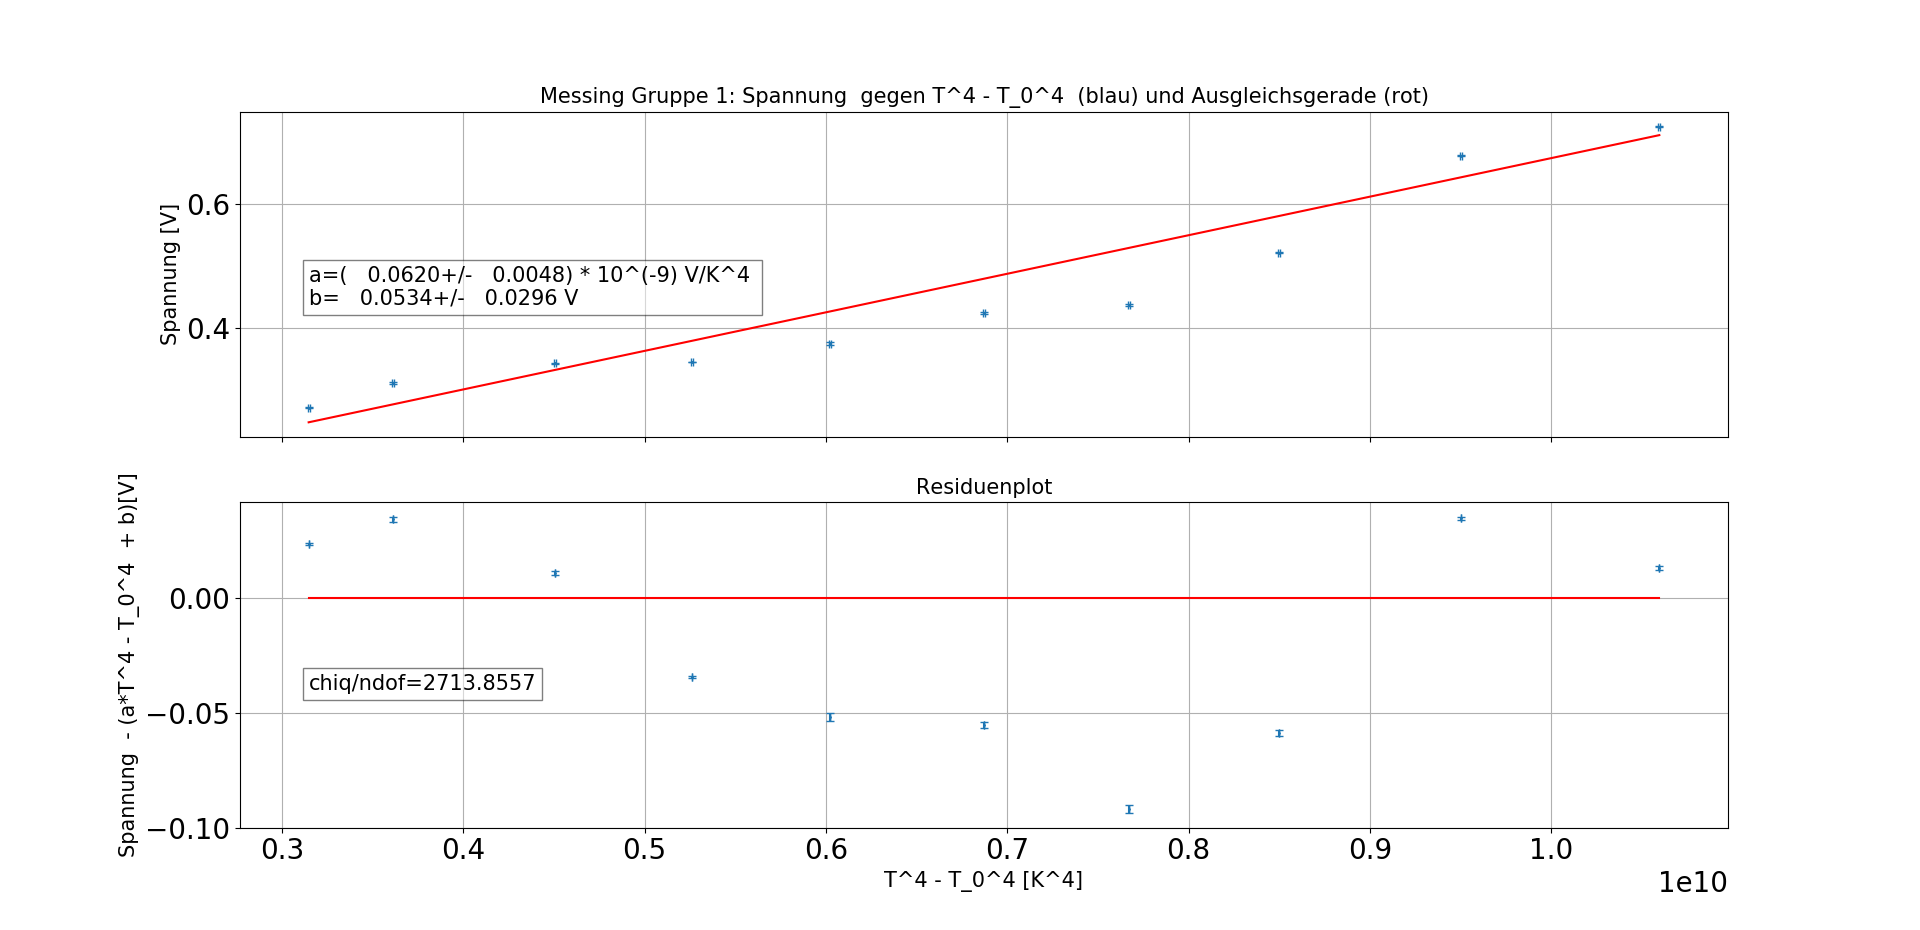
\includegraphics[scale=0.42]{Bilder/Gruppe1_Messing.png}%
	\caption[lineare Regression für die 1 Gruppe zur Messing-Seite]{lineare Regression für die 1 Gruppe zur Messing-Seite}%
	\label{pic:Abbildung 2}%
\end{figure}

\begin{figure}[H]
	\hskip -2 cm
	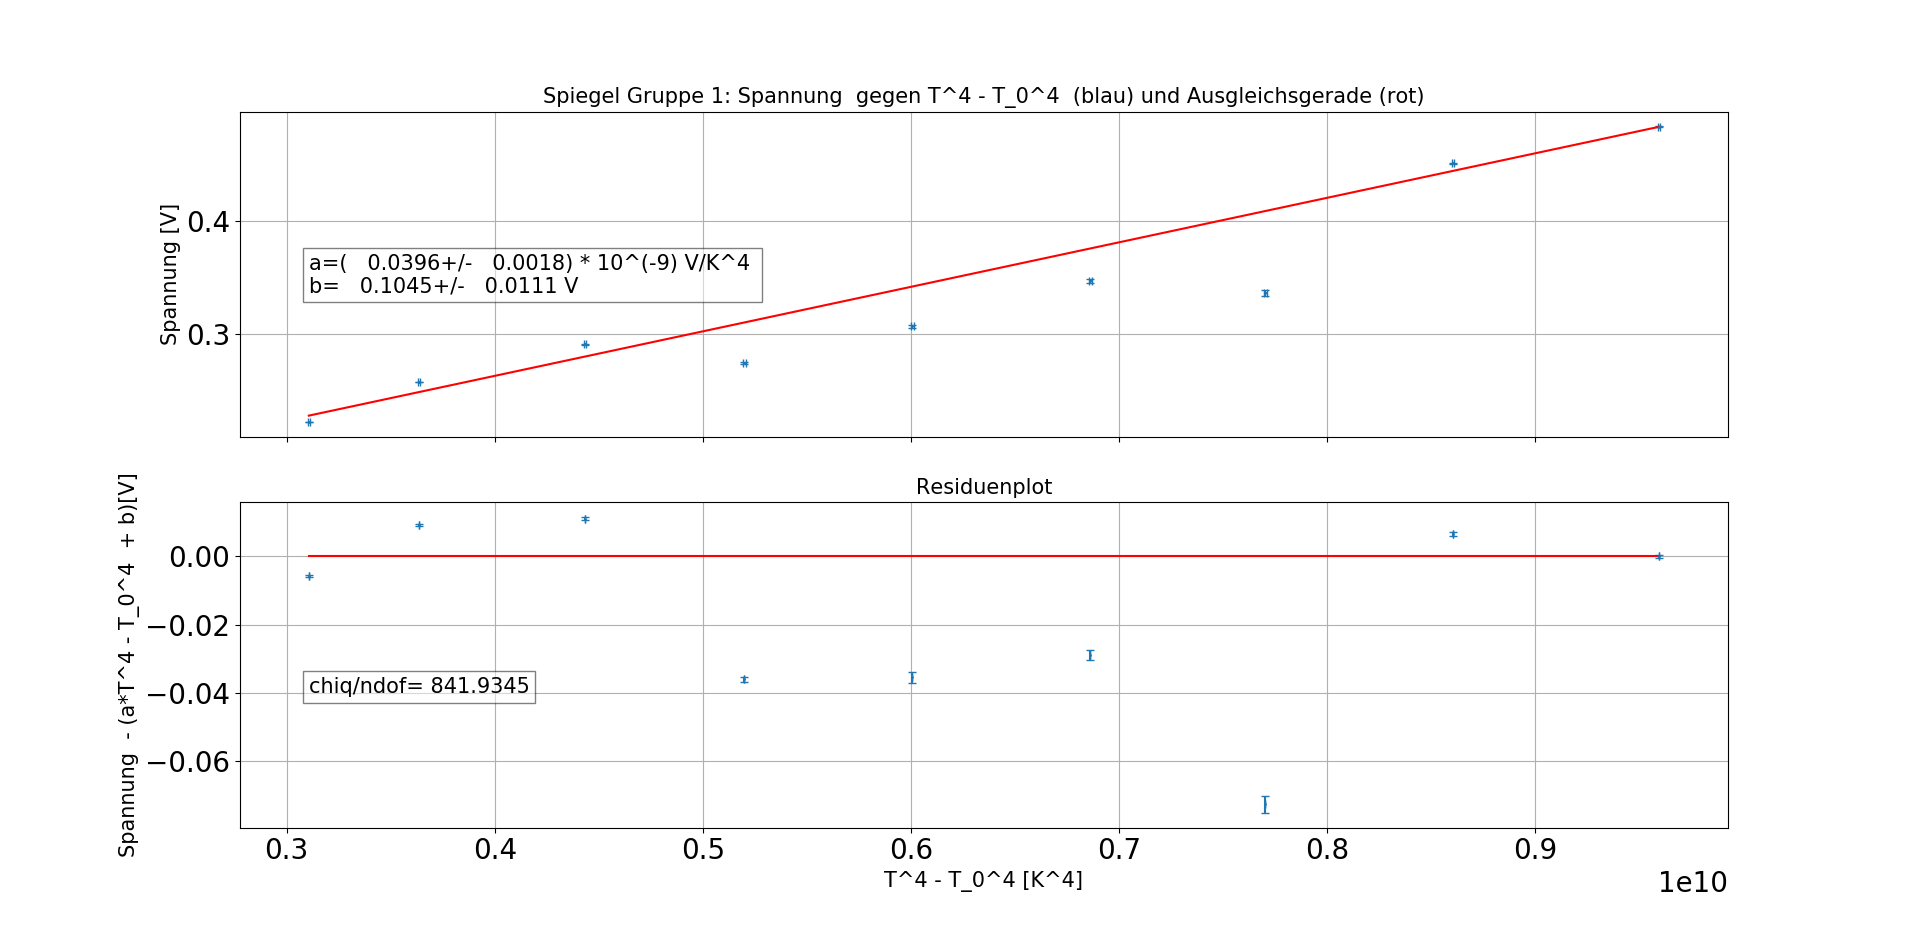
\includegraphics[scale=0.42]{Bilder/Gruppe1_Spiegel.png}%
	\caption[lineare Regression für die 1 Gruppe zur Spiegel-Seite]{lineare Regression für die 1 Gruppe zur Spiegel-Seite}%
	\label{pic:Abbildung 2}%
\end{figure}

\begin{figure}[H]
	\hskip -2 cm
	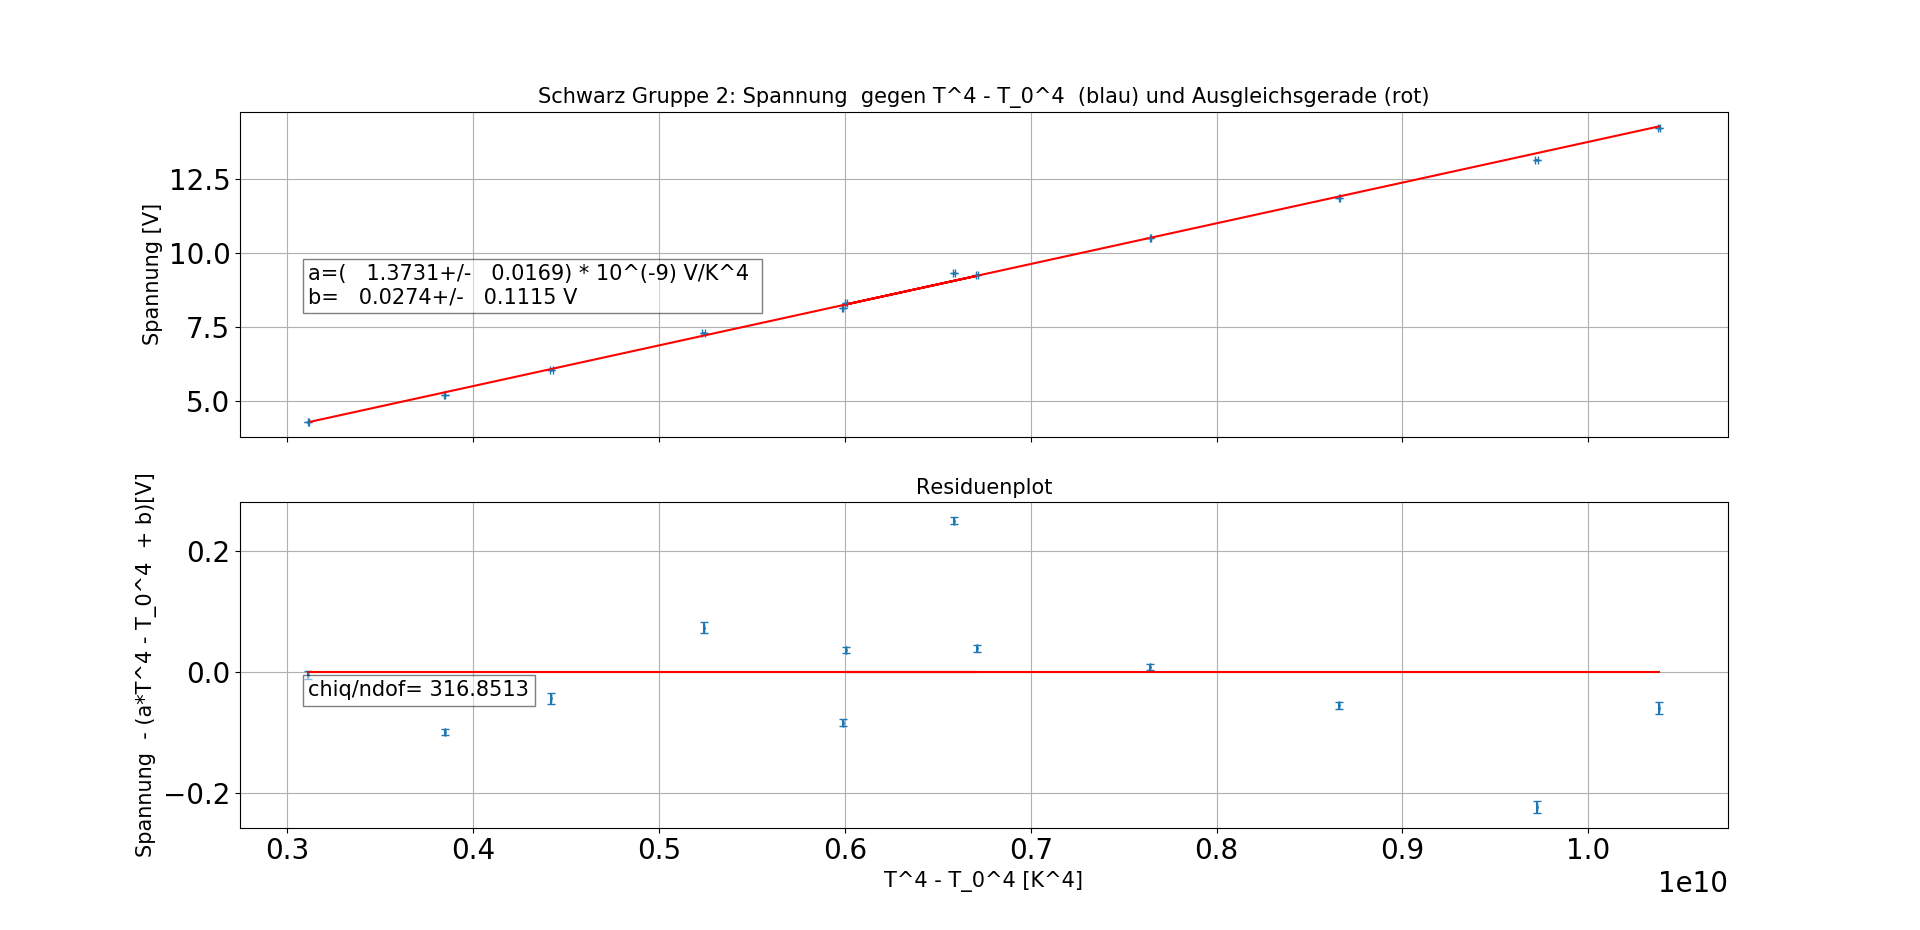
\includegraphics[scale=0.42]{Bilder/Gruppe2_Schwarz.png}%
	\caption[lineare Regression für die 2 Gruppe zur schwarzen Seite]{lineare Regression für die 2 Gruppe zur schwarzen Seite}%
	\label{pic:Abbildung 2}%
\end{figure}

\begin{figure}[H]
	\hskip -2 cm
	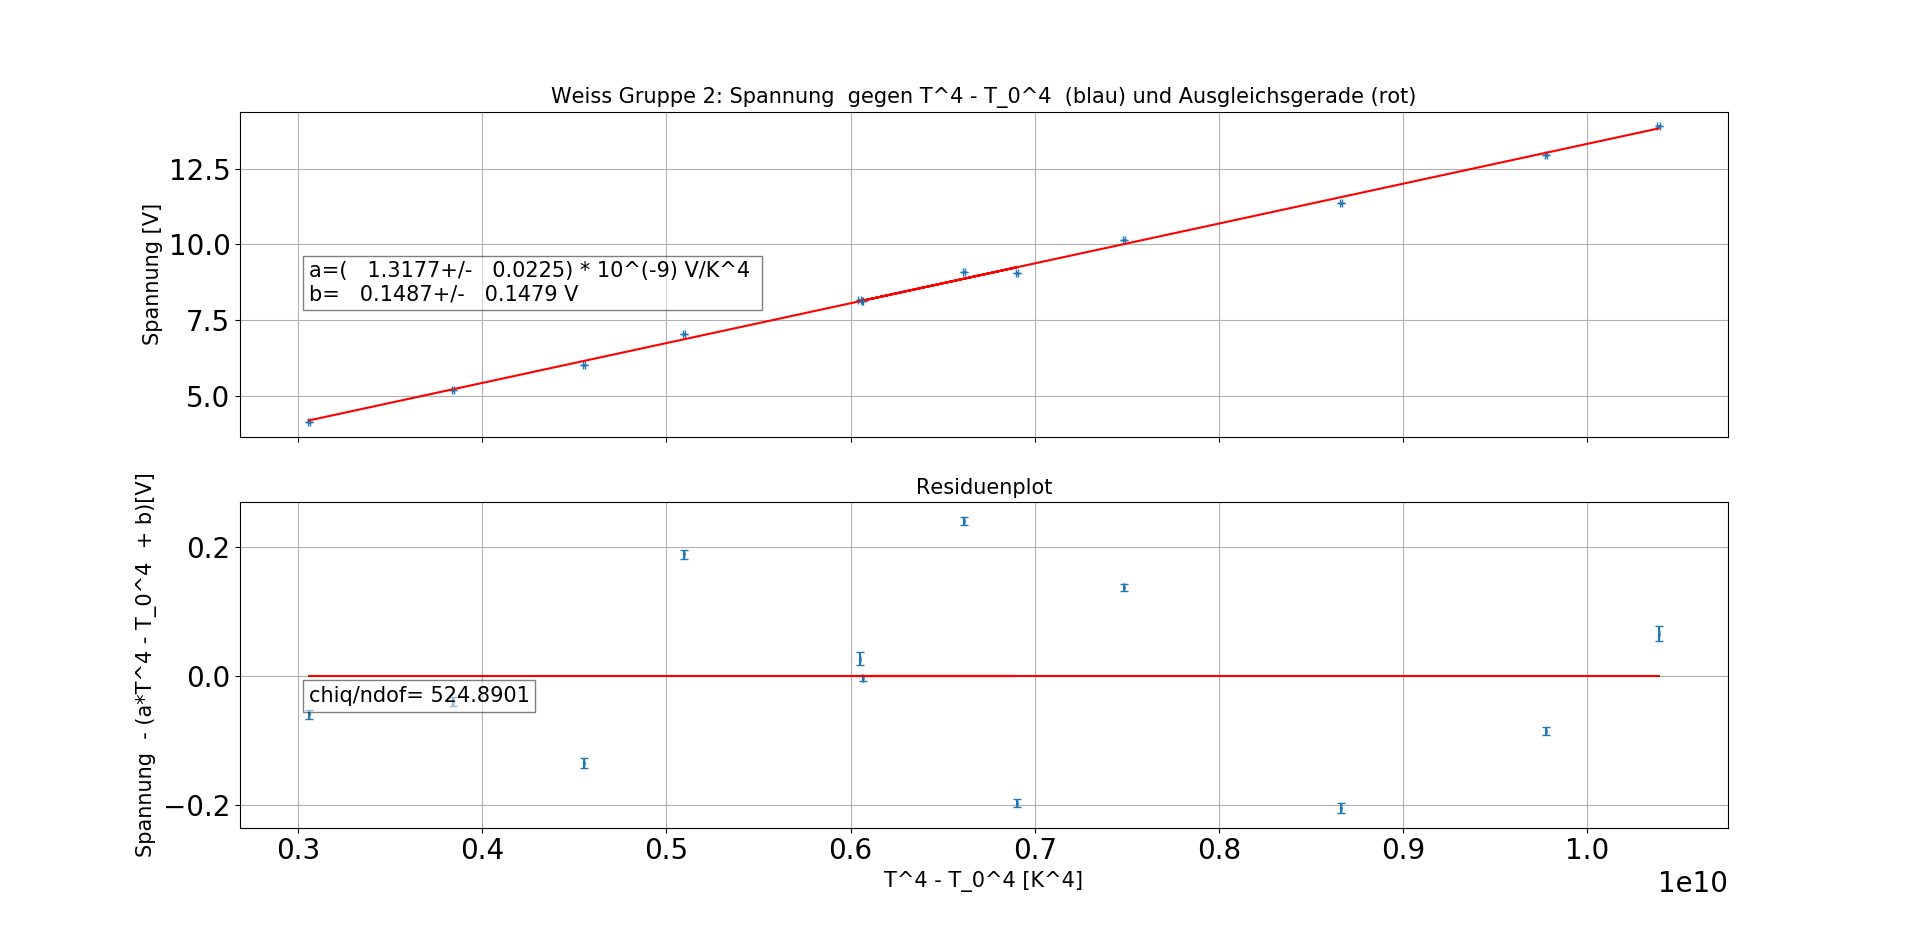
\includegraphics[scale=0.42]{Bilder/Gruppe2_Weiss.png}%
	\caption[lineare Regression für die 2 Gruppe zur weißen Seite]{lineare Regression für die 2 Gruppe zur weißen Seite}%
	\label{pic:Abbildung 2}%
\end{figure}

\begin{figure}[H]	
	\hskip -2 cm
	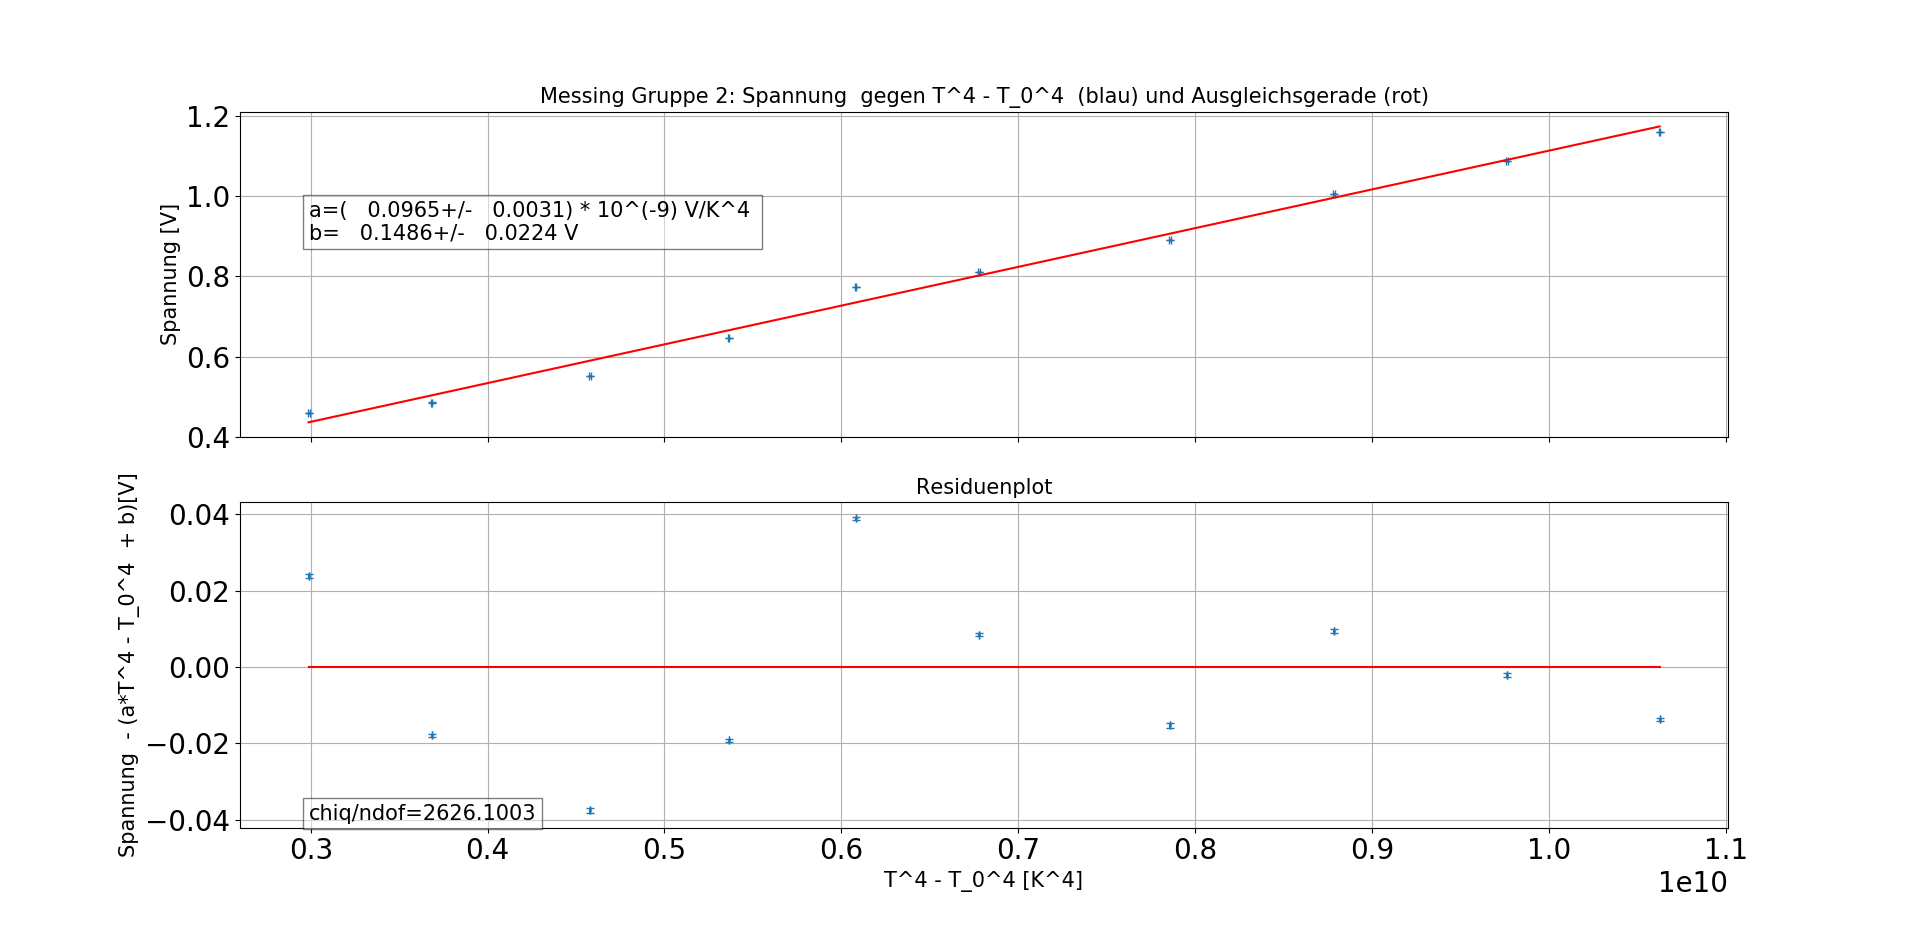
\includegraphics[scale=0.42]{Bilder/Gruppe2_Messing.png}%
	\caption[lineare Regression für die 2 Gruppe zur Messing-Seite]{lineare Regression für die 2 Gruppe zur Messing-Seite}%
	\label{pic:Abbildung 2}%
\end{figure}

\begin{figure}[H]
	\hskip -2 cm
	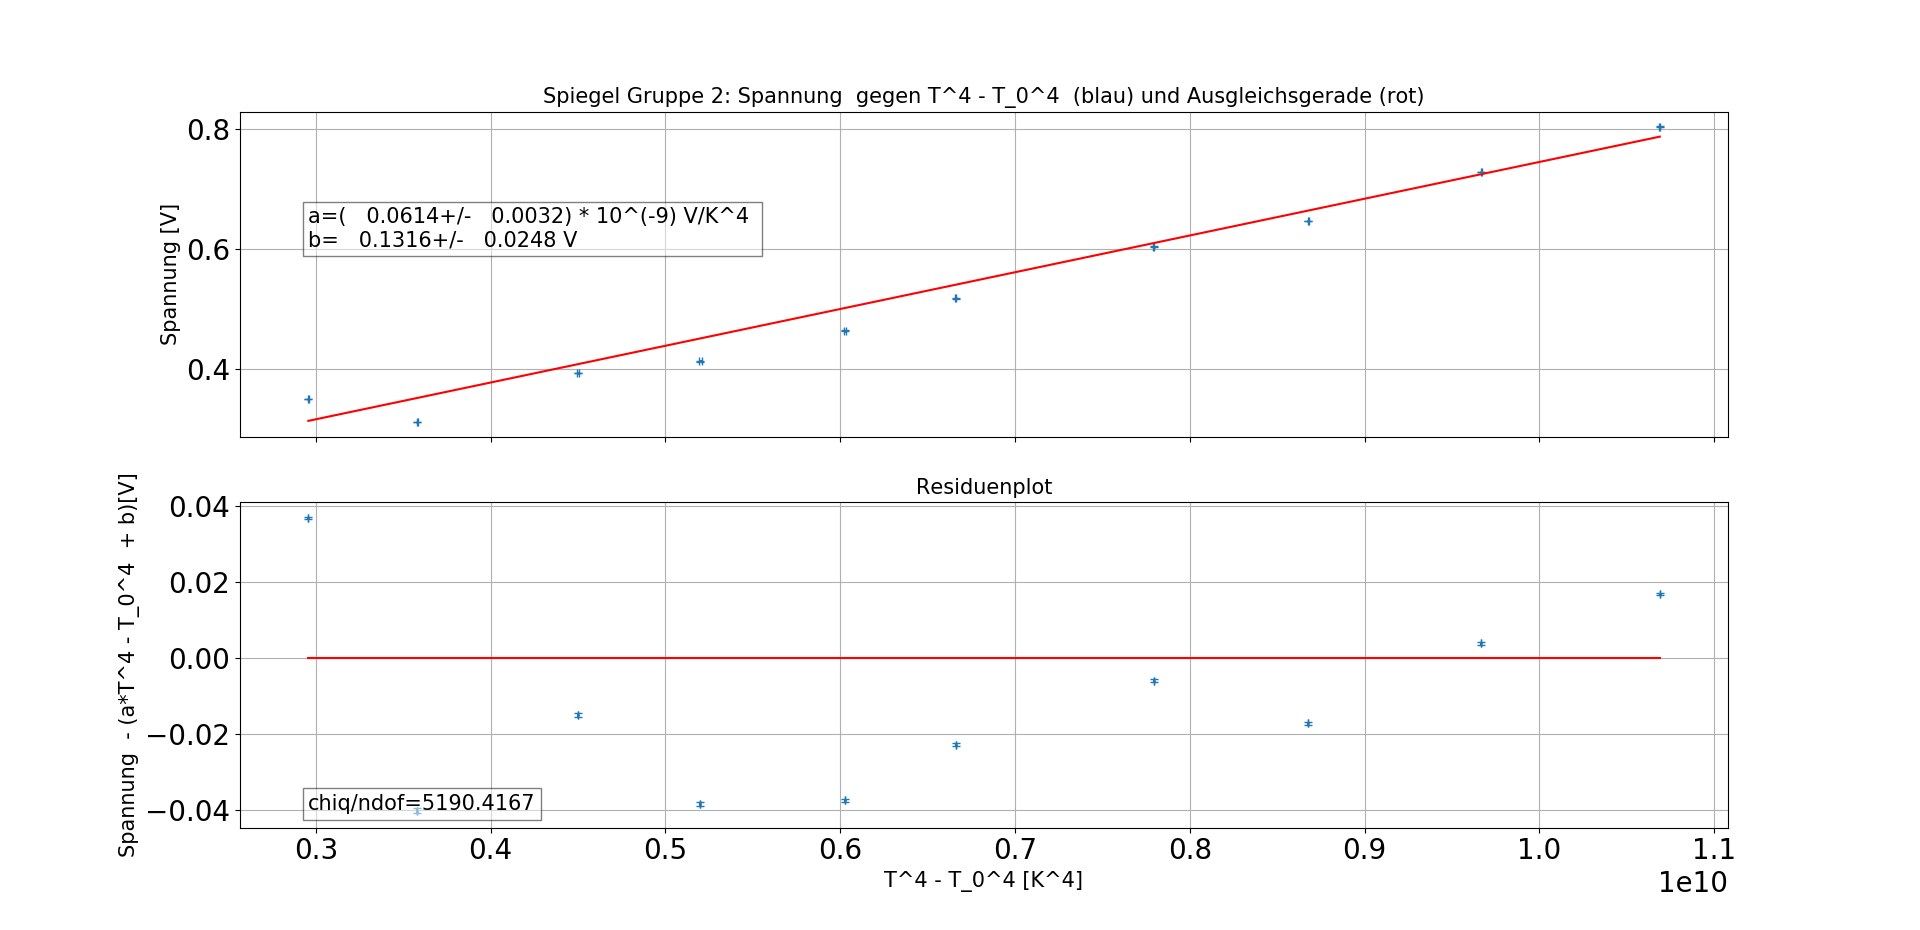
\includegraphics[scale=0.42]{Bilder/Gruppe2_Spiegel.png}%
	\caption[lineare Regression für die 2 Gruppe zur Spiegel-Seite]{lineare Regression für die 2 Gruppe zur Spiegel-Seite}%
	\label{pic:Abbildung 2}%
\end{figure}

\begin{figure}[H]
	\hskip -2 cm
	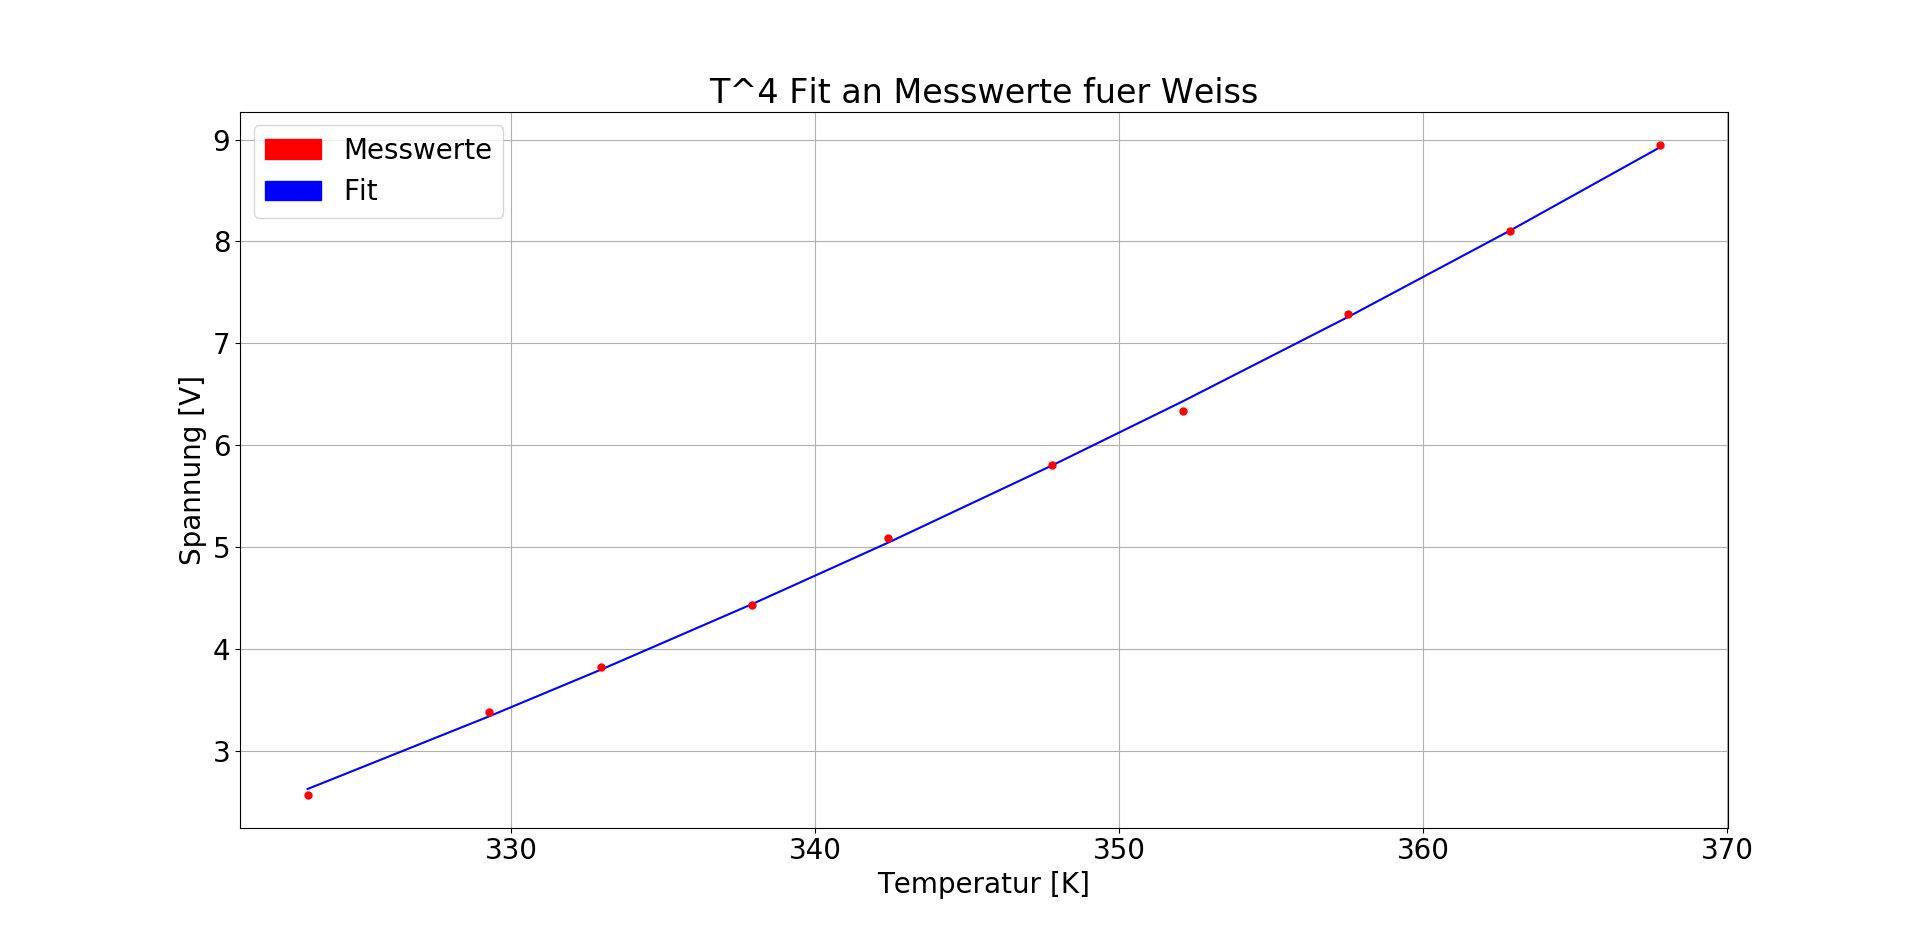
\includegraphics[scale=0.42]{Bilder/Gruppe1_Fit_Weiss.png}%
	\caption[$T^x$-Fit für die 1 Gruppe zur weißen Seite]{$T^x$-Fit für die 1 Gruppe zur weißen Seite}%
	\label{pic:Abbildung 2}%
\end{figure}

\begin{figure}[H]
	\hskip -2 cm
	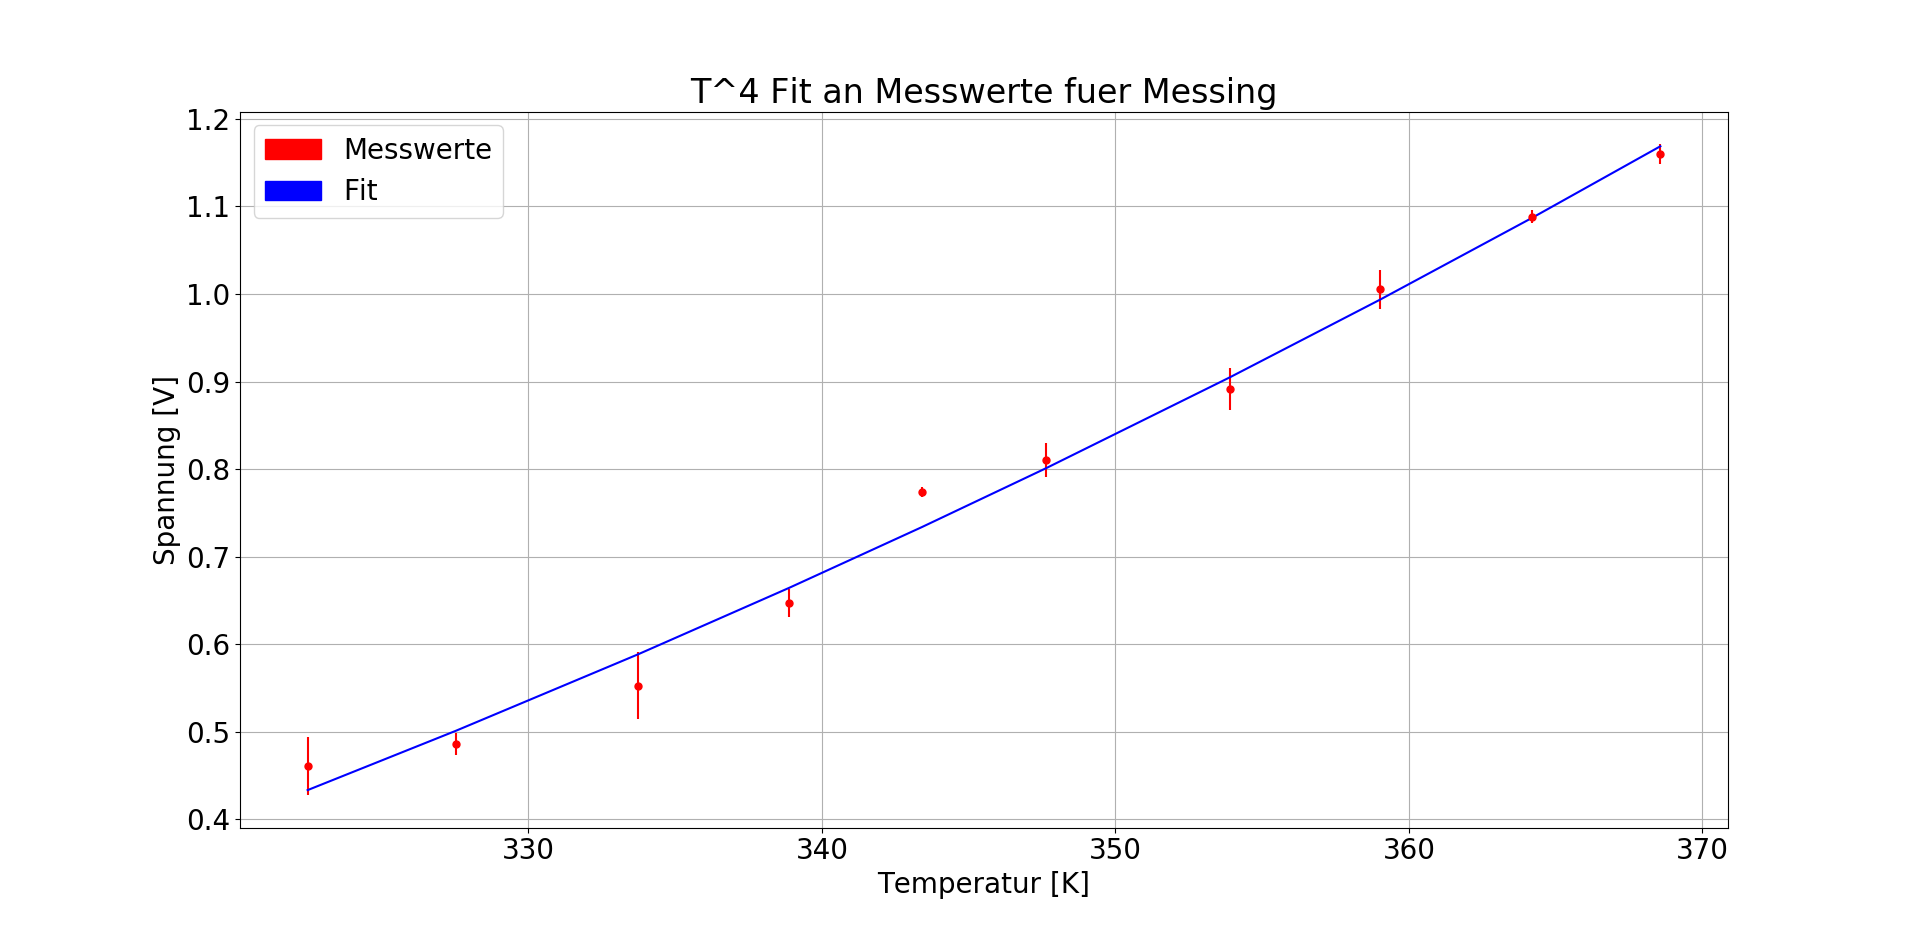
\includegraphics[scale=0.42]{Bilder/Gruppe2_Fit_Messing.png}%
	\caption[$T^x$-Fit für die 2 Gruppe zur Messing-Seite]{$T^x$-Fit für die 2 Gruppe zur Messing-Seite}%
	\label{pic:Abbildung 2}%
\end{figure}

\end{center}

\newpage
\listoffigures
\listoftables
\end{document}